\chapter{Instruments}
\label{chapter:inst}
\thispagestyle{myheadings}

\graphicspath{{Instruments/}}

\epigraph{The primary excitation mechanism of the aurora is provided by the entry of fast protons, possibly together with other positive ions, into the earth’s atmosphere. The primary electrons will be stopped at great heights and will not give a large contribution to the auroral luminosity.}{[NB: \textit{In situ} measurements by \citet{mcilwain1960} reversed the conclusions of the second sentence.] \citep{seaton1954}}

Auroral researchers put crowdsourced synchronized data acquisition into practice a century ago. 
Størmer set up several Norwegian schools and stations appropriately spaced for auroral stereography with cameras and telephones.
Størmer experimentally determined for the auroral forms he was interested in studying that cameras should be separated by at least \unit[20]{km} and optimally \unit[50]{km}, with wider separation for higher altitude aurora \citep{egeland2013} such as \unit[630.0]{nm} emissions.
Two previous experiments with \unit[3..5]{km} camera baseline range were unsuccessful with trigonometric stereography methods \citep{egeland2013}.
Figure~\ref{fig:stormersens}(b) shows the ill-conditioning that narrow-spaced auroral observatories suffer from, using Størmer's trigonometric method \citep{egeland2013}
\begin{equation}\label{eq:stormer}
h = d \frac{\sin\alpha \sin\beta}{\sin(\beta-\alpha)}
\end{equation}
where $h$ is altitude [km] of the auroral feature, $d$ is the distance [km] between observers, and $\alpha,\beta$ are the elevation angles to the auroral feature for each observer.
\begin{figure}\centering
	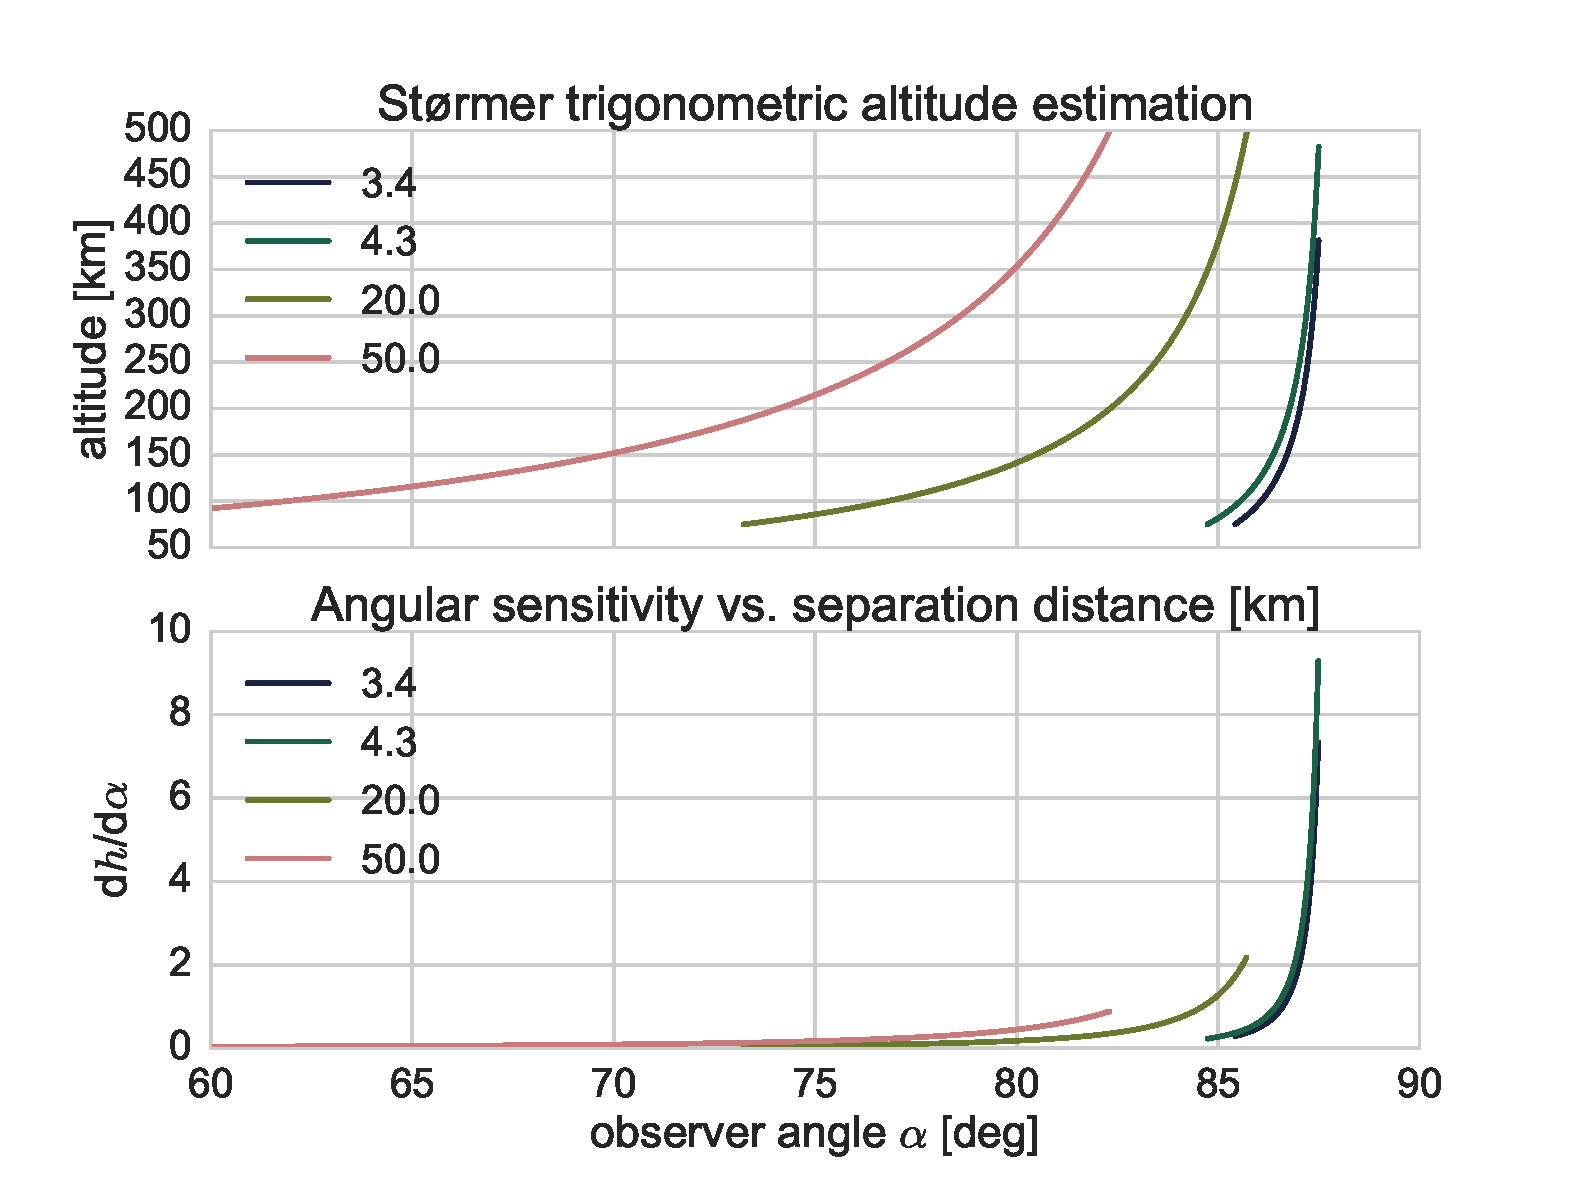
\includegraphics[width=\linewidth]{gfx/stormer_sens}
	\caption{(a) Solutions to \eqref{eq:stormer} for station spacing $x \in \lbrace 3.4, 4.3, 20,50 \rbrace$~km.
		(b) Derivative of \eqref{eq:stormer}, revealing problematic ill-conditioning for narrow-spaced observations.}
	\label{fig:stormersens}
\end{figure}
Considering Størmer's standard $40^\circ$ FOV camera \citep{egeland2013}, film print resolution, optically thin target biasing peak intensity and observer positional uncertainty, it would be difficult to get sufficient accuracy with sub-\unit[5]{km} spaced cameras, from the author's personal experience at these techniques with $9^\circ$ FOV digital cameras.
Timing uncertainty would be significant in Størmer's voice-synchronized \unit[200]{ms} exposure with human auditory-motor reaction time of an excellent athlete under ideal conditions at \unit[82]{ms} mean with \unit[17]{ms} standard deviation \citep{pain2007}.
Consider the profoundly cold outdoor conditions in northern Scandinavia with 1910-vintage clothing, finger slipping on the shutter button, shivering and the like.
It is probable that a mean delay of several hundred milliseconds with large standard deviation might have been the case for an ensemble of freezing students and adult photographers under such trying conditions.
This temporal inaccuracy would not be devastating for inverted-V aurora or other slow to moderate $B_\perp$ apparent speed morphologies.
For the narrow, fast-moving features studied by HiST, such mismatched synchronization would be completely intolerable.


Observational biases, ill-posed/ill-conditioned systems and other inherent remote sensing challenges both instrumental and mathematical, have often been limiting factors in advancing magnetosphere-ionosphere coupling theory.
\textit{In situ} sensing was vital to unlocking physical puzzles at the dawn of the space age and continues to be an essential component to unlocking the secrets of the fine structure of earth's magnetosphere.
Spatiotemporal ambiguities implicit in \textit{in situ} ionosphere and magnetosphere sensing are partially mitigated by close-flying formations of rockets \citep{lynch2012} and satellites \citep{parham2016}.
However, the ability to observe wide swathes of sky at high spatiotemporal resolution is vital to numerous important geospace problems.
An \textit{in situ} platform in motion will always have sampling ambiguities as the structure observed is changing in both space and time as the platform only measures one point in both space and time. 
There is a symbiosis as the \textit{in situ} sensing gives clues as to the particle kinetics responsible for auroral displays, and the ground-based instruments see a swath of sky, using a suitable forward model in the data inversion.

This chapter details the configuration and buildout of the DMC and HiST instruments. 
DMC was a proof-of-concept fielded prototype, observing multiple scales of aurora simultaneously as described in section~\ref{sec:dmc}.
The HiST instrument described in section~\ref{sec:hist} is a full-fledged auroral tomography system, yielding \unit[20]{ms} cadence estimates of auroral precipitation from approximately \unit[50..20000]{eV}, an energy range adequate to characterize Alfvénic aurora and to distinguish alternate particle acceleration mechanisms.
Chapter~\ref{chapter:sim} details the planning and modeling for the optimum \unit[1..10]{km} camera spacing of the HiST system. 
HiST uses robust numerical methods to overcome the ill-posed, ill-conditioned and non-uniqueness problems that frustrated Størmer a century ago.
The purpose of this chapter is to provide historical context of auroral remote sensing leading to HiST, review the state of the art of high-resolution auroral sensors, and describe two specific optical remote sensing systems (DMC/HiST) developed and deployed for the dissertation research.

\section{Auroral Observation Background}\label{sec:obshistory}
The earliest dedicated attempts to photograph aurora in the First Polar Year 1882--1883 was unsuccessful despite \unit[4]{min} exposures \citep{egeland2013}.
The first actual photograph of aurora in 1892 was of too poor quality for quantitative use \citep{egeland2013}.
J. Sýkora's spectrographic plates collected in 1899--1900 were the first quality spectrographic data \citep{chernouss2008}. 
Birkeland tried from 1898--1900 unsuccessfully to simultaneously photograph aurora with two cameras separated by \unit[3.4]{km}, and in 1910 Størmer failed to estimate auroral heights with \unit[4.3]{km} separation \citep{egeland2013} (NB: HiST phase 1 camera separation \unit[3.1]{km}).
Størmer's contributions from 1909 onward resulted in his \unit[0.2]{s} exposure camera carefully constructed to record wavelengths from infrared to UV \citep{stormer1932} becoming the standard camera for IPY 1932.
Hundreds of Størmer's cameras collected a half-million photos, of which tens of thousands were of science-quality \citep{egeland2013}.
Størmer's emphasis on collecting prompt auroral emissions with careful star-based plate scale registration from multiple synchronized cameras separated by about $\unit[20..100]{km}$ may be thought of as direct philosophical ancestors to the HiST system developed during the course of this dissertation.
The problems Størmer's team faced in parsing 500,000 images would have been alleviated by the auroral discriminator developments in chapter~\ref{chapter:discrim}.
Størmer noted that processing one night's image stacks took about a month to process \citep{egeland2013}.

Despite the numerous advances during his long life by himself and others in auroral observations, Størmer passed away before unsolved magnetospheric and ionospheric puzzles began to be resolved via \textit{in situ} sensing of the early satellites.
A 1953 crowdsourcing auroral observation effort using prepaid postcards was plagued by imprecision and inaccuracy of human sighted auroral feature az/el.
It was recognized that replicable, precisely registered, synchronized wide-field optical data was vital to understanding auroral correlation to ionospheric perturbations \citep{birkeland1908,stormer1930,stoffregen1955}.
Leading up to IGY 1957, a network of newly designed ``all-sky'' cameras synchronized with broadband HF receivers were deployed in and near the auroral oval region in Scandinavia.
This effort was designed for better quantification of auroral behavior vs. ionospheric perturbations known then to affect LF-VHF interactions in the ionosphere.
The stations, manufactured in $2\times2$~m huts used the \unit[50]{Hz} power grid via synchronous film-driving motors to ensure sufficiently tight synchronization of the all-sky video. 
A typical setup was \unit[7]{s} uniform exposure, chosen to avoid overexposure while still capturing weak aurora on the \unit[100]{line/mm} film, at \unit[1]{min.} cadence.
Although temporal aliasing was clearly evident in the film strips, this aliasing was a compromise chosen for the great cost of the film required for months to years of observation.
The star registration vital to making altitude estimates of aurora were based on methods by \citet{stormer1930} as updated using current technology.
Deployment of all-sky cameras more extensively about the north and south auroral ovals led quickly to conclusions on the geomagnetic alignment of aurora and the diurnal behavior of the oval versus solar zenith angle \citep{denholm1961}.
The THEMIS all-sky camera network across North America has provided numerous new geophysical insights as used with its satellite--all-sky pairing as well as ISR and rocket experiments \citep{donovan2006}.
The upcoming frame rate improvements via the tREX system \citep{liang2016} will provide a new generation of insights from a medium frame-rate imaging network added to the continent-wide THEMIS ASI network through Canada and Alaska.
HiST phase 2 deployments may include coördinated observations with the tREX/THEMIS network.

A great challenge across STEM disciplines in general and the geosciences specifically is the storage and processing of vast amounts of data over constrained CPU and data bandwidth resources.
The first digital image scanner in 1957 could not hold the 2 bit, $176 \times 176$ pixel image in its \unit[6]{kB} memory, and so the persistence of a scanning oscilloscope phosphor provided the assembled image for human visual appreciation \citep{kirsch1958}.
Over a decade later, the forefront of automated microscope slide processing was an extensively customized computer constructed in a collaboration between multiple US Federal agencies.
This ``Spectre II'' automated cytometry machine was capable of $256 \times 256$ pixel 8-bit resolution, with a single image unable to fit in the \unit[16]{kB} memory \citep{shapiro1969}.
The data reduction employed by Spectre II overcame the issue of a full digitized multi-chromatic microscope slide consuming \unit[62.5]{GB} of storage.
At the time that amount of tape storage would have been over \unit[1200]{km} in length \citep{shapiro1969}, stretching from the earth's surface to over the top of the ionosphere if held vertical.
A contemporary IBM System/360 Model 91 mainframe used by NASA for the Apollo missions had a \unit[16]{MHz} CPU and \unit[2]{MB} of RAM \citep{ibm1967}.
Such computing power was not available in commodity desktop PC form until the late 1980s.
It was not until the 1990s that computer-controlled auroral observation systems with digital storage became common \citep{bjornthesis}.
Computers and hard drives after 2010 (see section~\ref{sec:prochistory}) were finally fast enough to sustain all-night operations from a full-frame, \unit[50]{fps} camera, a key requirement for distinguishing the acceleration mechanism behind plasma turbulence associated with multiple particular auroral forms.

CCD cameras began integration into astronomy in the 1970s \citep{lynds1975} and gradually digital imaging began taking over nearly all aspects of science and personal photography over the next three decades as challenges of imaging efficiency were resolved \citep{monet1993}.
In the past decade, the value of scientific CMOS (sCMOS) cameras has been proven for the high resolution high speed imaging. 
Cooled sCMOS cameras generally exceed the performance of CCD cameras for many applications.
In the most photon-starved regimes, EMCCD cameras reign supreme, as in the HiST system, which like Størmer's system a century before targets prompt emissions from UV to IR.


\section{Dual Multiscale Camera (DMC)}\label{sec:dmc}
Aurora simultaneously evolves on $B_\perp$ scale widths from micro $\sim \unit[10]{m}$ to global $\sim \unit[1000]{km}$.
Within this auroral scale width range there is a continuüm of process scales continually evolving.
Instruments such as THEMIS are designed to observe the auroral oval across the width of North America simultaneously, but at low frame rate with all-sky FOV.
The ASK instrument observes with $3^\circ$ FOV at multiple narrowband wavelengths.
A key novelty of DMC was the simultaneous bandstop prompt emission filtered observation at \unit[33]{ms} cadence at $50^\circ$ and $6^\circ$ FOVs, from a single site.

DMC was constructed in part using cameras obtained for prior experiments such as Mishap and earlier work, funded under NSF EAGER contract \#FA9550-11-1-0356.
Running \$40K each EMCCD and sCMOS cameras designed for clean lab biological operations in short bursts for fluorescence microscopy is quite different than running for 12 hour stretches each night in a shed or box.
The Mishap system \citep{plant2011} deployed in 2011 near Fairbanks, AK experienced significant difficulty with dropped frames and lost timing of frames, using the system timing diagram of Figure~\ref{fig:mishap}.
\begin{sidewaysfigure}
    \includegraphics[page=2,width=0.95\linewidth]{gfx/ProposedTimingSystem}
    \caption{Mishap timing system block diagram form 2010-2011.}\label{fig:mishap}
\end{sidewaysfigure}
Some of these issues were algorithmic, and some were due to the single-core Intel Core 2 Duo E7500 CPU used in Mishap versus the far more powerful quad-core Intel Sandy Bridge i7-2600K CPU used for DMC and the even more powerful quad-core Intel Haswell i7-4790 CPU used for HiST.
As is inherently the case, little insight is gained when comparing different CPU architectures based on clock speed, particularly with on-chip GPUs in processors as modest as the \$25 Raspberry Pi allowing full-screen HD video playback and recording.
Intel Sandy Bridge and newer CPUs made numerous architecture changes \citep{lempel2011}, of which a few are particularly important for high-speed scientific video recording and processing, including:
\begin{enumerate}
    \item elimination of Front Side Bus (bottleneck for RAM and PCI Express cards)
    \item per \#1, bringing the memory controller onto the CPU die
    \item AVX SIMD floating point math-large improvements in automatic vectorization of for loops and other parallelizable problems
\end{enumerate}
The efficiency gains for math operations common to DMC/HiST gave at least a five-fold improvement in processing time.
The same is true for the TRANSCAR energy deposition modeling discussed in section~\ref{sec:fwd}.

The DMC instrument was conceived as a dual-purpose mission:
\begin{enumerate}
    \item test imaging and processing technology essential to HiST functionality
    \item explore correlations between microscale (\unit[0.1..1]{m} width) and mesoscale $\gg \unit[1]{km}$ auroral structure on \unit[20]{ms} timescales
\end{enumerate}
More specifically, DMC mission goals included:
\begin{enumerate}
	\item Two cameras successfully run at full speed for 8 hours, with data rates approaching \unit[500]{MB/s}
	\item Two cameras frame synchronized to better than $\unit[10^{-3}]{s}$
	\item Autonomous system controlled remotely from Internet bandwidth as low as \unit[5]{kB/sec} and latencies $ > \unit[250]{ms}$, using open-source tools
	\item Timing LED device (binary counter) to verify that system doesn't drop or duplicate frames, and that two separate PCs/Cameras are synchronized to specification
	\item Fully automated scheduler (runs without human intervention till hard drives fill)
    \item Sends daily start/stop recording emails, posts logs
	\item online updates with current images posted every $N=60$ seconds
    \item Many debug/disable/error points conveniently located in code
	\item Measured CPU usage during data acquisition $< 10$\%
	\item 16-bit raw grayscale data preserved with lossless compression
	\item actual experiment configuration for each recording stored in XML headers (human-readable) detailing many pertinent camera and algorithm settings, for science and engineering analysis
	\item Programs kept simple enough for research outreach, bringing students quickly to do meaningful work on parts of the program
	\item Data headers human-readable, data format easily accessible via open-source tools.
\end{enumerate}
These mission goals were met and the robustness of the HiST system was greatly improved by having the critical concepts tested in a real field system before deploying the significantly more complicated HiST stations.

\FloatBarrier
\subsection{DMC Build and Deployment}
The benchtop setup of DMC is shown in Figure~\ref{fig:dmcbench}.
\begin{figure}\centering
	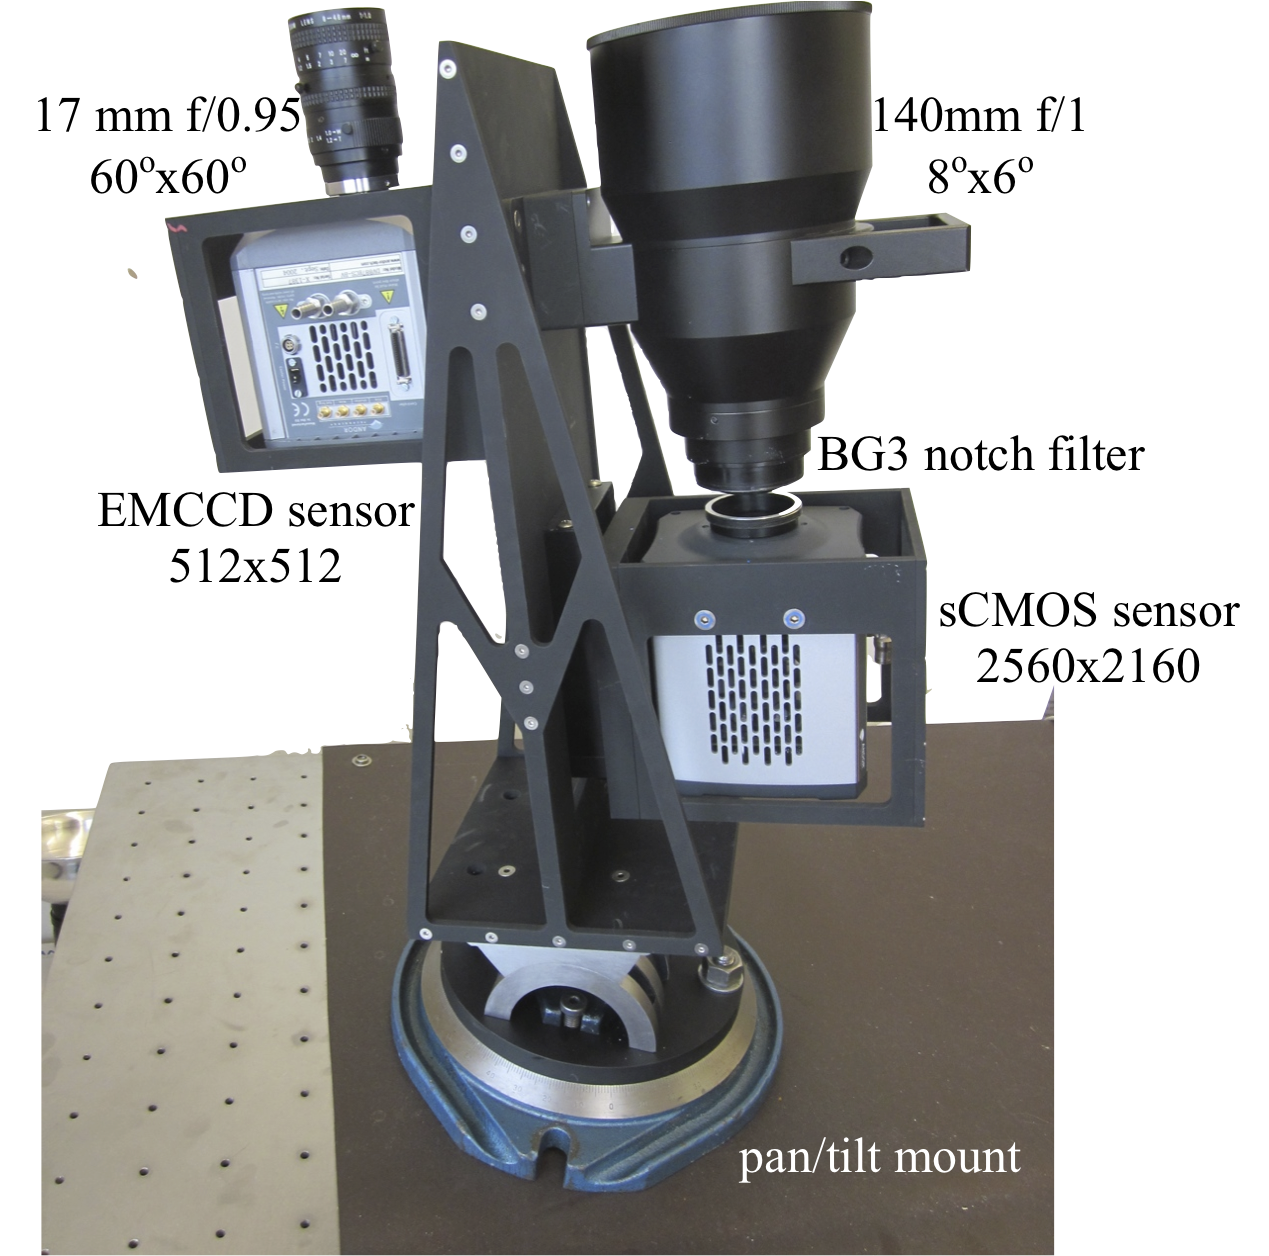
\includegraphics[width=\linewidth]{gfx/DMC_bench1}
	\caption{DMC benchtop setup. 
		At left is iXon EMCCD camera with a \unit[17]{mm} lens yielding a $50^\circ$ usable FOV. 
		At right is Neo sCMOS with 140mm lens yielding $6^\circ$ FOV. 
		Both cameras employ BG3 bandstop filters.
		The pan/tilt mount was fixed to be approximately centered on local magnetic zenith, and was constructed by Heitor Murato and Glenn Thayer of BU SIF.}
	\label{fig:dmcbench}
\end{figure}
The iXon camera at left had a usable FOV of $50^\circ \times 50^\circ$ and the Neo camera at right had a usable FOV of $6^\circ \times 8^\circ$.
Both cameras were BG3 filtered as in Figure~\ref{fig:BG3trans} to select prompt emissions as described in section~\ref{sec:physicsemissions}.
It was discovered upon deployment under the dome at Søndrestrøm that the dome was acting as a lens in the near field of the large aperture \unit[140]{mm} Neo lens.
This was confirmed by removing the dome as in Figure~\ref{fig:nodome}, which immediately gave ideal focus.
A flat glass aperture was promptly constructed and installed by Eggert Guðmundsson and crew as depicted in Figure~\ref{fig:dmcflat}.
\begin{figure}\centering
	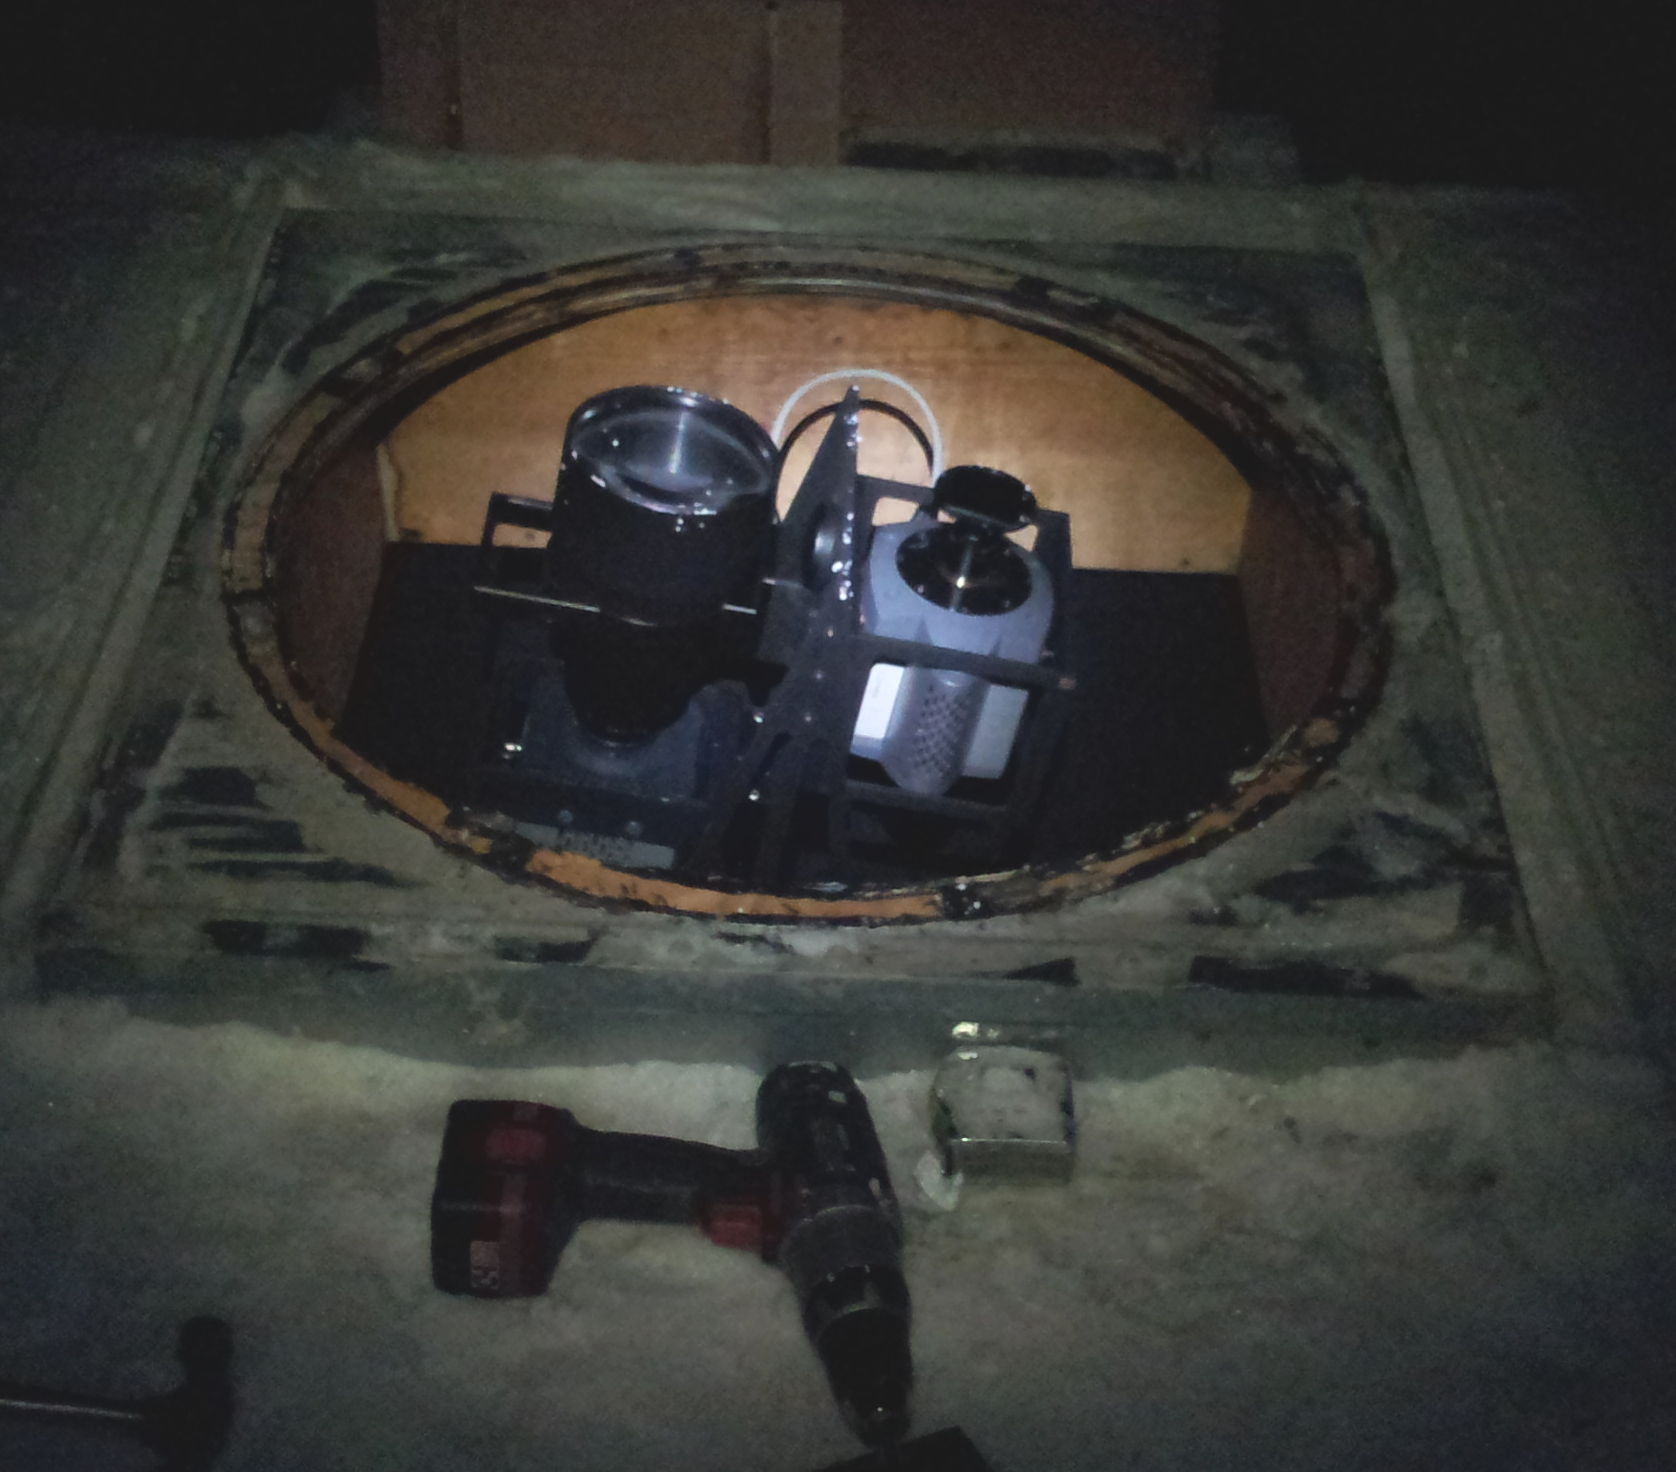
\includegraphics[width=\linewidth,trim=0 500 0 200,clip]{gfx/DMC_deployed_nodome}
	\caption{DMC installation at Søndrestrøm with dome removed for testing.}
	\label{fig:nodome}
\end{figure}
\begin{figure}\centering
	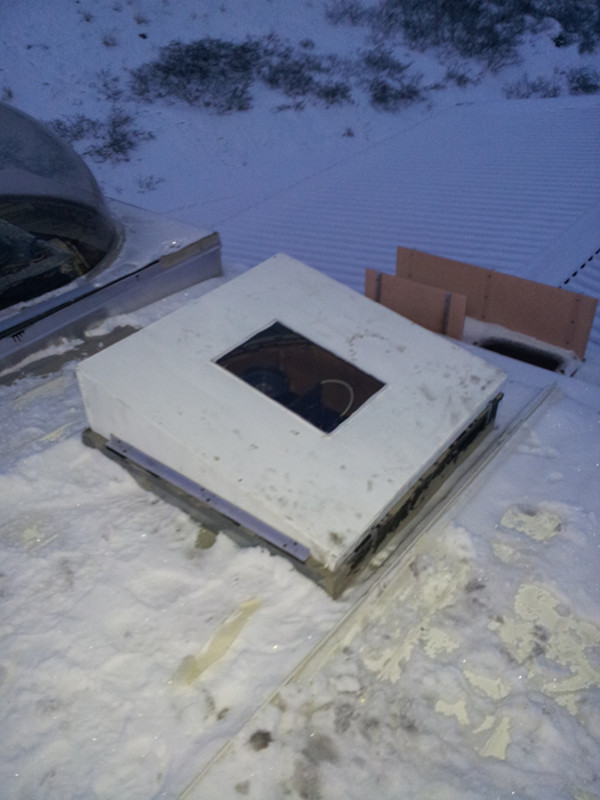
\includegraphics[width=\linewidth,trim=0 200 0 200,clip]{gfx/DMC-opening}
	\caption{DMC installation at Søndrestrøm with flat glass aperture, giving best possible focus.}
	\label{fig:dmcflat}
\end{figure}
Despite old-age failure and repair of the iXon camera and initial severe issues with the Neo camera driver, the DMC instrument was successful and has supported additional multi-instrument experiments.
DMC remains on site and ready to serve at Søndrestrøm ISR.


\FloatBarrier
\subsection{DMC Data}
DMC quickly yielded interesting data, which has been archived and will be exploited in future work.
Once DMC was working, the focus shifted to HiST build and deployment to take advantage of the same auroral season.
A sample of the novel data coming from DMC is given in Figure~\ref{fig:dmcsplit}.
\begin{figure}
	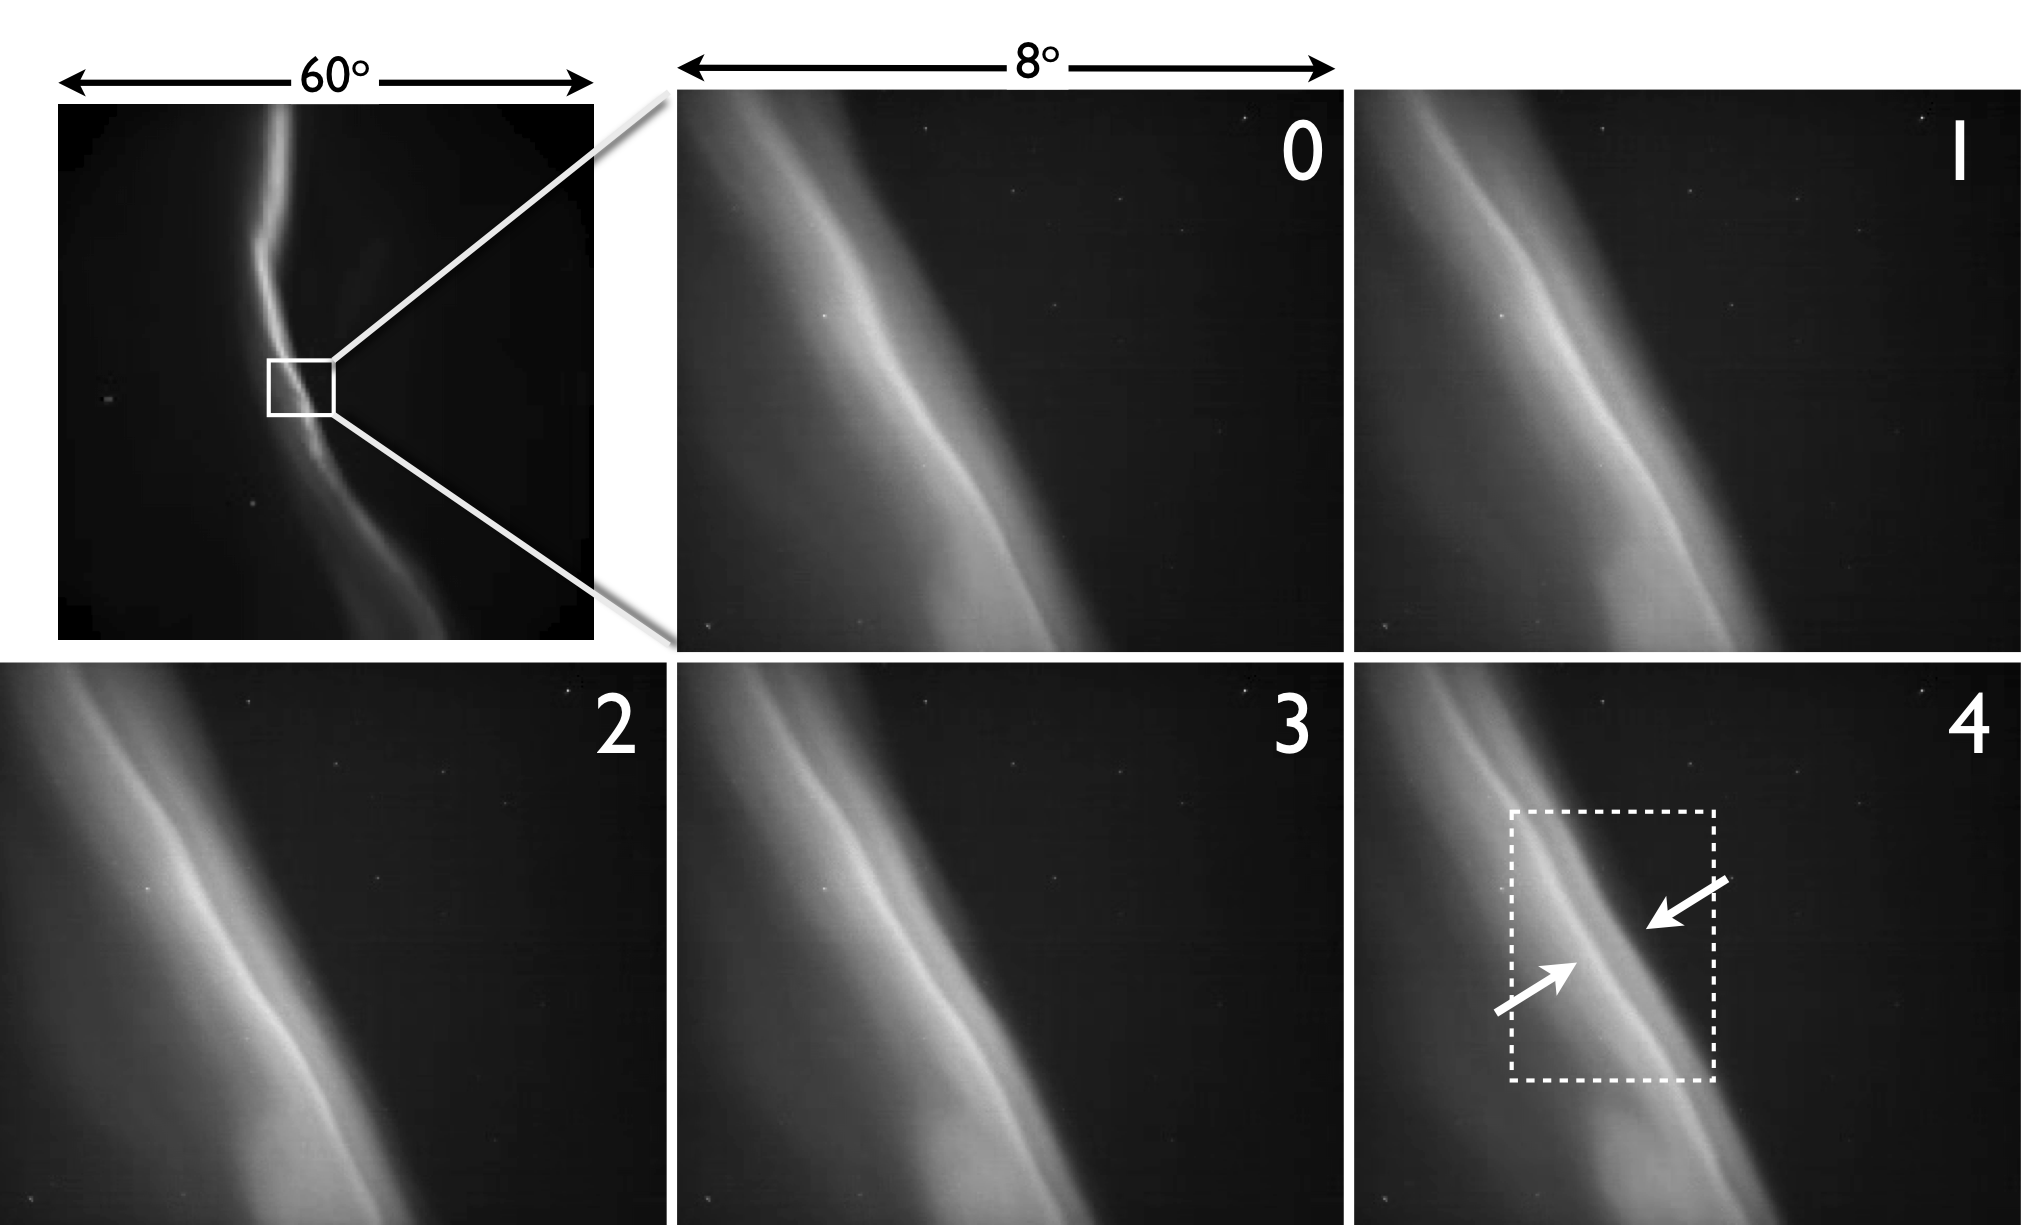
\includegraphics[width=\linewidth]{gfx/DMC_samples}
	\caption{Example of multiscale insights from DMC on 13 JAN 2013. The upper-left wide FOV images comes from the EMCCD at \unit[33]{fps}, while the \unit[50]{fps} Neo sequence in subpanels 0-4 reveals the fine scale structure invisible to the wide field camera.}
	\label{fig:dmcsplit}
\end{figure}
The splitting arc evolution of \unit[200]{m} width in Figure~\ref{fig:dmcsplit} requires tomographic analysis to quantify the Alfvén wave-driven precipitation causing the arc.
A splitting arc was observed with HiST and PFISR and is analyzed in section~\ref{sec:split}.
Another spitting auroral arc was observed with the cropped image sequence in Figure~\ref{fig:dmcsplit2}.
\begin{sidewaysfigure}
	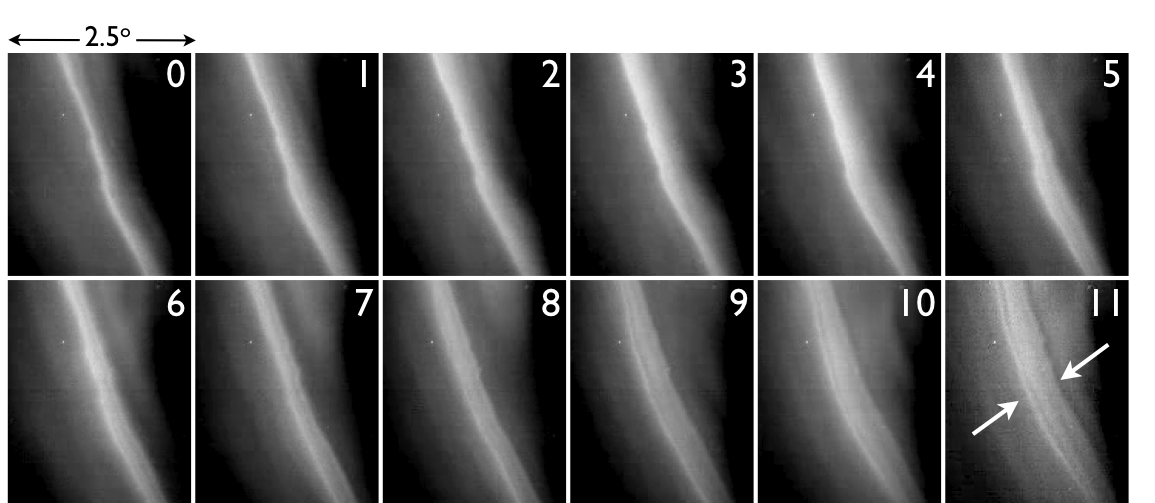
\includegraphics[width=\linewidth]{gfx/packet}
	\caption{Evolution of splitting arc as observed by Neo sCMOS narrowfield camera. The faint splitting structure would likely be washed out and smeared over by \unit[557.7]{nm} and \unit[630.0]{nm} emissions if not for the bandstop BG3 filter employed.}
	\label{fig:dmcsplit2}
\end{sidewaysfigure}
This fine structure would be completely missed in a widefield camera due to the fine sub-\unit[100]{m} structure.
Finally, a filamentary auroral arc that could come from inverted-V aurora and/or Alfvénic accelerated electrons is shown in Figure~\ref{fig:dmcfil}.
\begin{sidewaysfigure}
	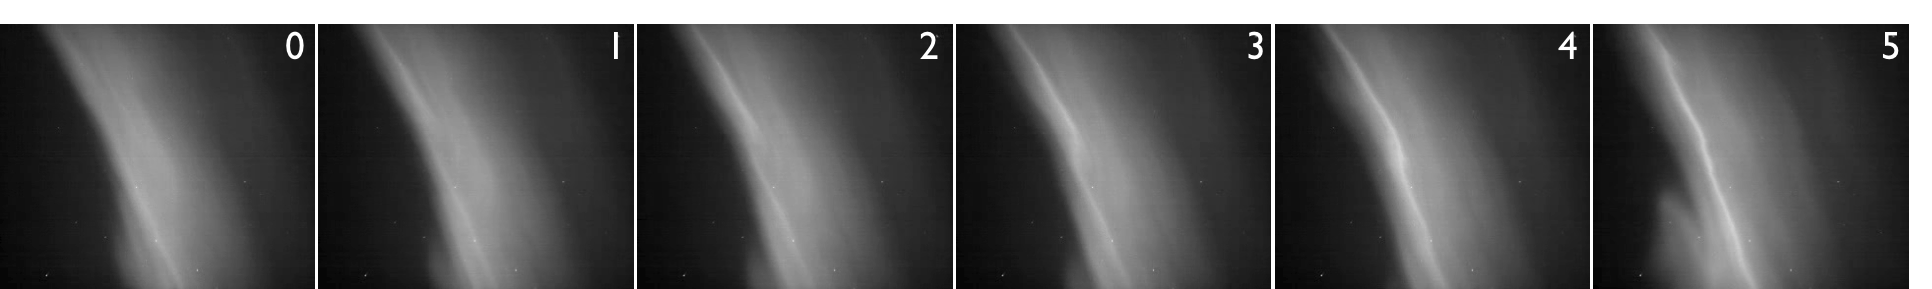
\includegraphics[width=\linewidth]{gfx/filament}
	\caption{Filamentary arc observed by DMC. Determining source acceleration would require a system like HiST to provide differential number flux estimates vs. time.}
	\label{fig:dmcfil}
\end{sidewaysfigure}
Determining source acceleration would require a system like HiST to provide differential number flux estimates vs. time.
These examples are a small taste of the data archived. 
Using the algorithms refined with HiST for joint ISR-optical analysis, future work is anticipated to analyze the single-site cameras data with Søndrestrøm ISR data.
The fast plasma line receiver estimates of electron density will be useful for recent data collected as another data fusion input \citep{vierinen2016}.

As an initial interpretation of these data, it is well established that field-aligned bursts of low energy electron precipitation occur at the edges of dynamic auroral forms. 
ISR measurements have identified anomalous ionospheric turbulence in these regions \citep{akbari2012}. 
\citet{akbari2013} revealed that this edge turbulence appears in thin layers at ranges where the ionospheric density gradients become zero (e.g., the F-region peak, and E-to-F region transition trough). 
Initial DMC observations have revealed a subtle optical signature in this region that appears as a damped outward propagating wave with wavelength $\sim \unit[300]{m}$ in Figure~\ref{fig:dmcsplit2}. Further accumulation of data will establish whether this is a consistent feature at auroral edges; and, finally, systematic comparison with space-borne and ground-based measurements will establish the electrodynamic context of these features and their consequences for communications, navigation, and high-latitude radar discrimination.

%\FloatBarrier
\subsection{Neo Burst Performance Characteristics}
Previous experiments \citep{dahlgren2013} had the operator sitting up all night waiting for aurora to press Record.
This level of human effort is not sustainable in the long term.
Obviously this method misses the build up time to interesting events, and stands a good chance of missing the desired events as well.
Nonetheless, this is how much high-speed auroral observation has taken place prior to about 2010.

For \citet{dahlgren2013} to achieve usable frame rates at full resolution, burst mode was used.
Burst mode uses the on-board camera memory in a short burst, upon which recording stops and the camera RAM is read to the PC RAM over the 3-tap Cameralink interface.
Neither binning or reducing width (width is the 2560 pixel dimension) helps improve frame rates.
Measurements were taken in Table~\ref{tab:neofullburst} at full frame.
\unit[$10^{-5}$]{s} is the minimum possible exposure time of Neo, which is much too short for auroral observations.
\unit[$10^{-3}$]{s} is roughly the minimum useful exposure time for aurora.
\unit[$10^{-2}$]{s} is about the fastest rate the companion iXon would run at. 
At full frame, the iXon can image at \unit[33]{ms} rate.
\begin{table}\centering
	\caption{Andor Neo full-frame burst imaging characteristics}\label{tab:neofullburst}
	\begin{tabular}{p{5em}p{4.5em}p{4.5em}p{5.5em}p{5em}p{5em}}
		\toprule
		Exp. Time (sec.) &  Width (pixels) & Height (pixels) &  Frames / sec &  Max \# of frames &  Max. Burst Time (sec.) \\
		\midrule
		$10^{-5}$ & 2560 & 2160 & 48.95 & 160 & 3.27 \\
		$10^{-3}$ & 2560 & 2160 & 46.68 & 160 & 3.43 \\
		$10^{-2}$ & 2560 & 2160 & 32.87 & 160 & 4.87 \\
		\bottomrule
	\end{tabular}
\end{table}
To optimize viewing area versus frame rate, the data in Table~\ref{tab:neooptburst} was collected.
Neo burst mode performance is optimized by exploiting Neo sCMOS sensor read geometry (center outward)--center on sensor.
\begin{table}\centering
	\caption{Neo burst performance with less than full-height image}\label{tab:neooptburst}
	\begin{tabular}{p{5em}p{4.5em}p{4.5em}p{5.5em}p{5em}p{5em}}
		\toprule
		Exp. Time (sec.) & Width (pixels) & Height (pixels) & Frames / sec & Max \# of frames & Max. Burst Time (sec.) \\
		\midrule
		$10^{-5}$ & 2560 & 1000 & 103.79 & 344 & 3.31\\
		$10^{-5}$ & 2560 & 512 & 197.58 & 667 & 3.38\\
		$10^{-5}$ & 2560 & 256 & 375.64 & 1315 & 3.5\\
		\midrule
		$10^{-3}$ & 2560 & 1000 & 94.12 & 344 & 3.65\\
		$10^{-3}$ & 2560 & 512 & 165.26 & 667 & 4.04\\
		$10^{-3}$ & 2560 & 256 & 273.82 & 1315 & 4.8\\
		\midrule
		$10^{-2}$ & 2560 & 1000 & 67.53 & 344 & 5.09\\
		$10^{-2}$ & 2560 & 512 & 79.87 & 667 & 8.35\\
		$10^{-2}$ & 2560 & 256 & 88.33 & 1315 & $\rightarrow\infty$\\
		\bottomrule
	\end{tabular}
\end{table}
From Table~\ref{tab:neooptburst} and the lens chosen, useful video is not obtained outside of \unit[5]{s} bursts. 
A sustainable mode of operation preserving FOV but sacrificing the excess resolution was required for the DMC mission.

%\FloatBarrier
\subsection{Neo Sustained Recording Performance Characteristics}
The Andor Neo sustained data rates are \textit{substantially} lower than burst mode rates due to the limited 3-tap Cameralink bandwidth.
The Andor Zyla 10-tap Cameralink has significantly higher frame rates than Neo with same sCMOS sensor.
Binning (creating macropixels by grouping adjacent pixels) is the key to sustained useful recording with the Andor Neo.
The maximum sustained frame rate with the Andor Neo using Solis 4.29.30012.0 is given in Table~\ref{tab:neomax}.
The Neo frame rates at 4x4 and 8x8 binning are comparable with the Andor iXon full frame rate.
\begin{table}\centering
	\caption{Neo maximum sustained frame rate with binning}\label{tab:neomax}
	\begin{tabular}{ccc}
		\toprule
		binning & width x height & frames / sec \\
		\midrule
		1x1 & 2560 x 2160 & 20 \\
		2x2 & 1280 x 1080 & 32 \\
		4x4 & 640 x 540 & 54 \\
		8x8 & 320 x 270 & 109 \\
		\bottomrule
	\end{tabular}
\end{table}


%\FloatBarrier
\subsection{Andor Neo DMC Resolution}
The Andor Neo camera has excess resolution for the planned FOV, so the Neo was typically binned 8x8.
An example of the excellent resolution of a splitting auroral arc at these Neo settings is given in Figure~\ref{fig:neosplit}.
\begin{figure}
	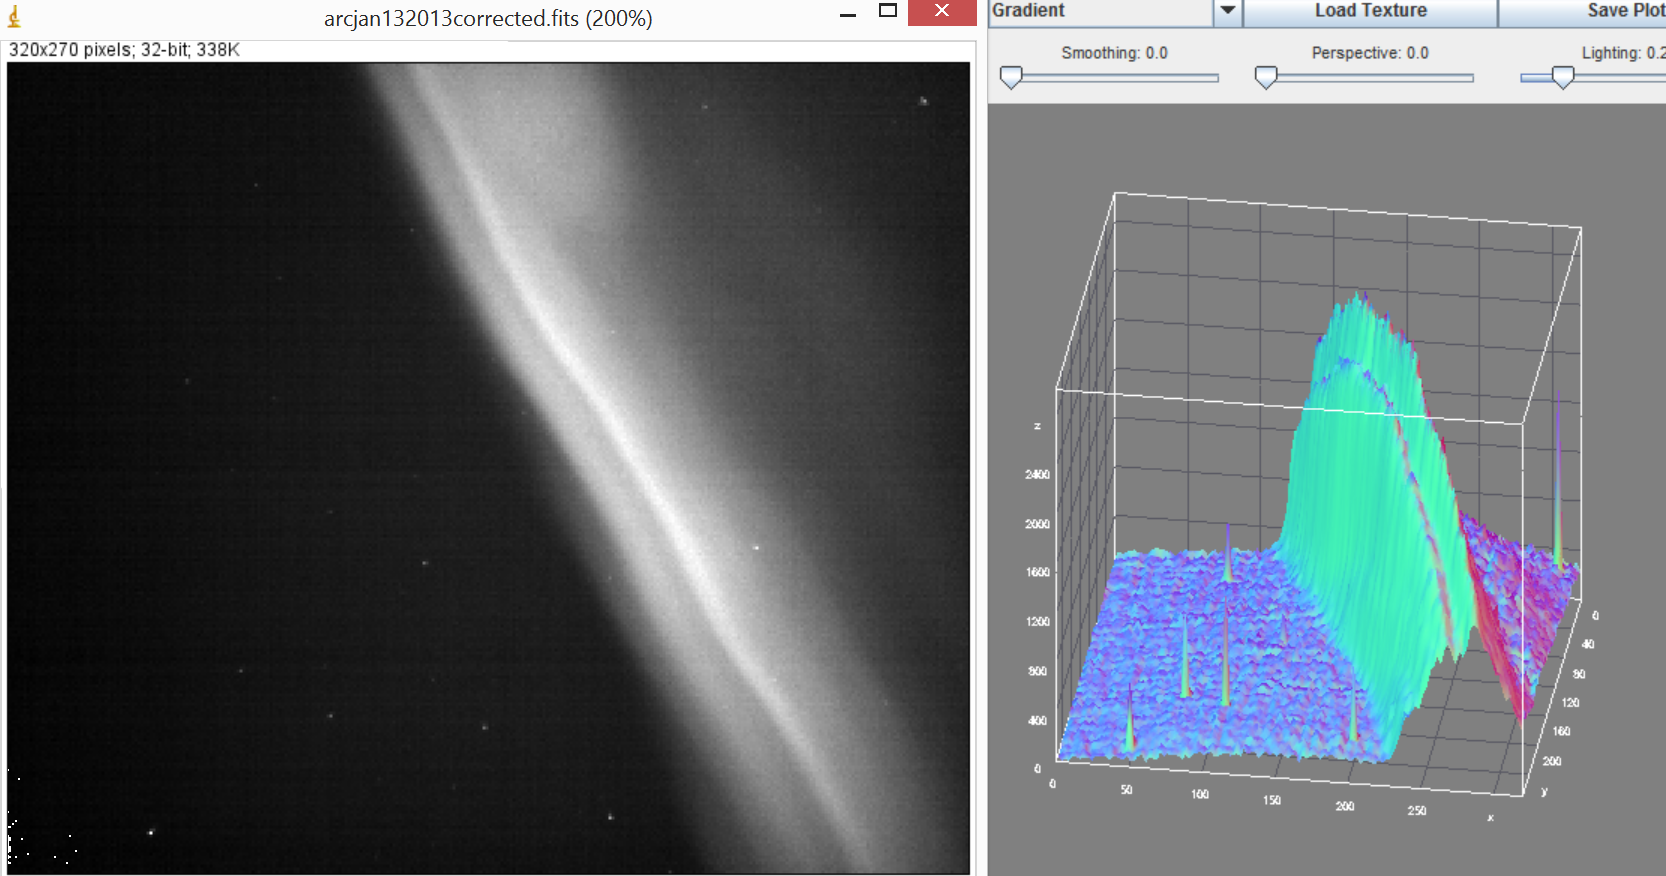
\includegraphics[trim=0 0 50 40,clip,width=\linewidth]{gfx/2013-01-13gradient}
	\caption{Splitting arc seen by DMC Neo camera, Jan 13, 2013}\label{fig:neosplit}
\end{figure}
The 3-D view of image intensity seen in the right panel of Figure~\ref{fig:neosplit} shows the fine quality of the focus and resolution with stars appearing as isolated peaks that stay nearly constant from one frame to the next.


\FloatBarrier
\subsection{Andor iXon DMC performance}
The Andor iXon 897 EMCCD (ca. 2003, serial X-1387, EEPROM ver. 6) used for DMC, like the Neo, was a camera reused from earlier projects.
As an EMCCD camera, with the iXon, objects totally invisible to eye \& Fourier analysis on Neo or Zyla can be seen in fine detail with iXon 897 under low-light conditions.
A comparison of important specification between the Neo and iXon is given in Table~\ref{tab:neoixon}.
\begin{table}\centering
	\caption{Comparison of important specification between iXon and Neo}\label{tab:neoixon}
	\begin{tabular}{rcc}
		\toprule
		Item: & iXon 897 & Neo \\
		\midrule
		Photo-electron sensitivity & $<1$ & 2.5 \\
		Pixels (w x h) & 512 x 512 & 2560 x 2160 \\
		Pixel size (microns) & 16 & 6.5 \\
		Sensor size (mm) & 8.2 x 8.2 & 16.6 x 14.0 \\
		Binning & on-chip & software \\
		Binning helps FPS? & YES & NO \\
		Reducing Width helps FPS? & NO & NO  \\
		Reducing Height helps fps, nearest: & bottom of sensor & center of sensor \\
		Minimum air cooling (deg. C) & -40 & -30 \\
		\bottomrule
	\end{tabular}
\end{table}
Images near the magnetic zenith tend to be the brightest by~\eqref{eq:bint}, so wide dynamic range is necessary. 
Because HiST and DMC work several degrees away from magnetic zenith, and faint structures embedded in bright structure is important.
Recent advances in EMCCD technology, after DMC was deployed have taken away the frame rate advantage of the sCMOS cameras for the moment.
HiST is known to have observed faint highly dynamic aurora, just above the noise floor.
These dynamic auroral forms are too faint for the Neo or Zyla sCMOS cameras to detect above the higher noise floor of the sCMOS instrument.
The higher resolution of sCMOS is useful for hyperspectral imagers like LiCHI \citep{goenka2016} that need four simultaneous images.


\section{HiST}\label{sec:hist}
While many of the algorithms and physics details of HiST are described in chapter~\ref{chapter:sim}, we briefly recount key aspects of HiST observations.
Following the successful startup of DMC as described in section~\ref{sec:dmc}, the HiST system final design and build commenced.
The goal of HiST and this dissertation is quantifying fine spatiotemporal auroral drivers, which are themselves of fine spatiotemporal structure.
Extensive forward modeling was carried out to optimize cameras positions as in Figure~\ref{fig:camres} and using theory consistent with optical and ISR observations in \citet{akbari2013}.
As confirmed by DMC experiences and with the new availability of the \unit[50]{fps}-capable iXon Ultra camera, only EMCCD cameras were used for HiST to maximize sensitivity with 16-bit dynamic range.

The initial HiST deployment was carried out by BU postdoc Hanna Dahlgren and then PhD candidates Chhavi Goenka and Hassan Akbari.
The second HiST camera was installed at the MF radar site in an outdoor, non-climate controlled box as shown in Figure~\ref{fig:hst2}.
\begin{figure}\centering
	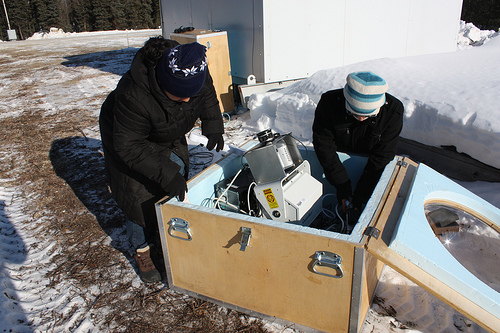
\includegraphics[width=0.9\linewidth]{gfx/HST1}
	\caption{HiST1 camera installation at the MF radar site in non-climate controlled box.}
	\label{fig:hst2}
\end{figure}
The blue insulation in this box was a help at night but a hindrance during the day, when temperatures rose to the order of $50^\circ$C.
This result led to detailed thermodynamic modeling for the climate control and cabinet system design for HiST Phase 2, as shown in Figure~\ref{fig:hist2cab}.
\begin{figure}
	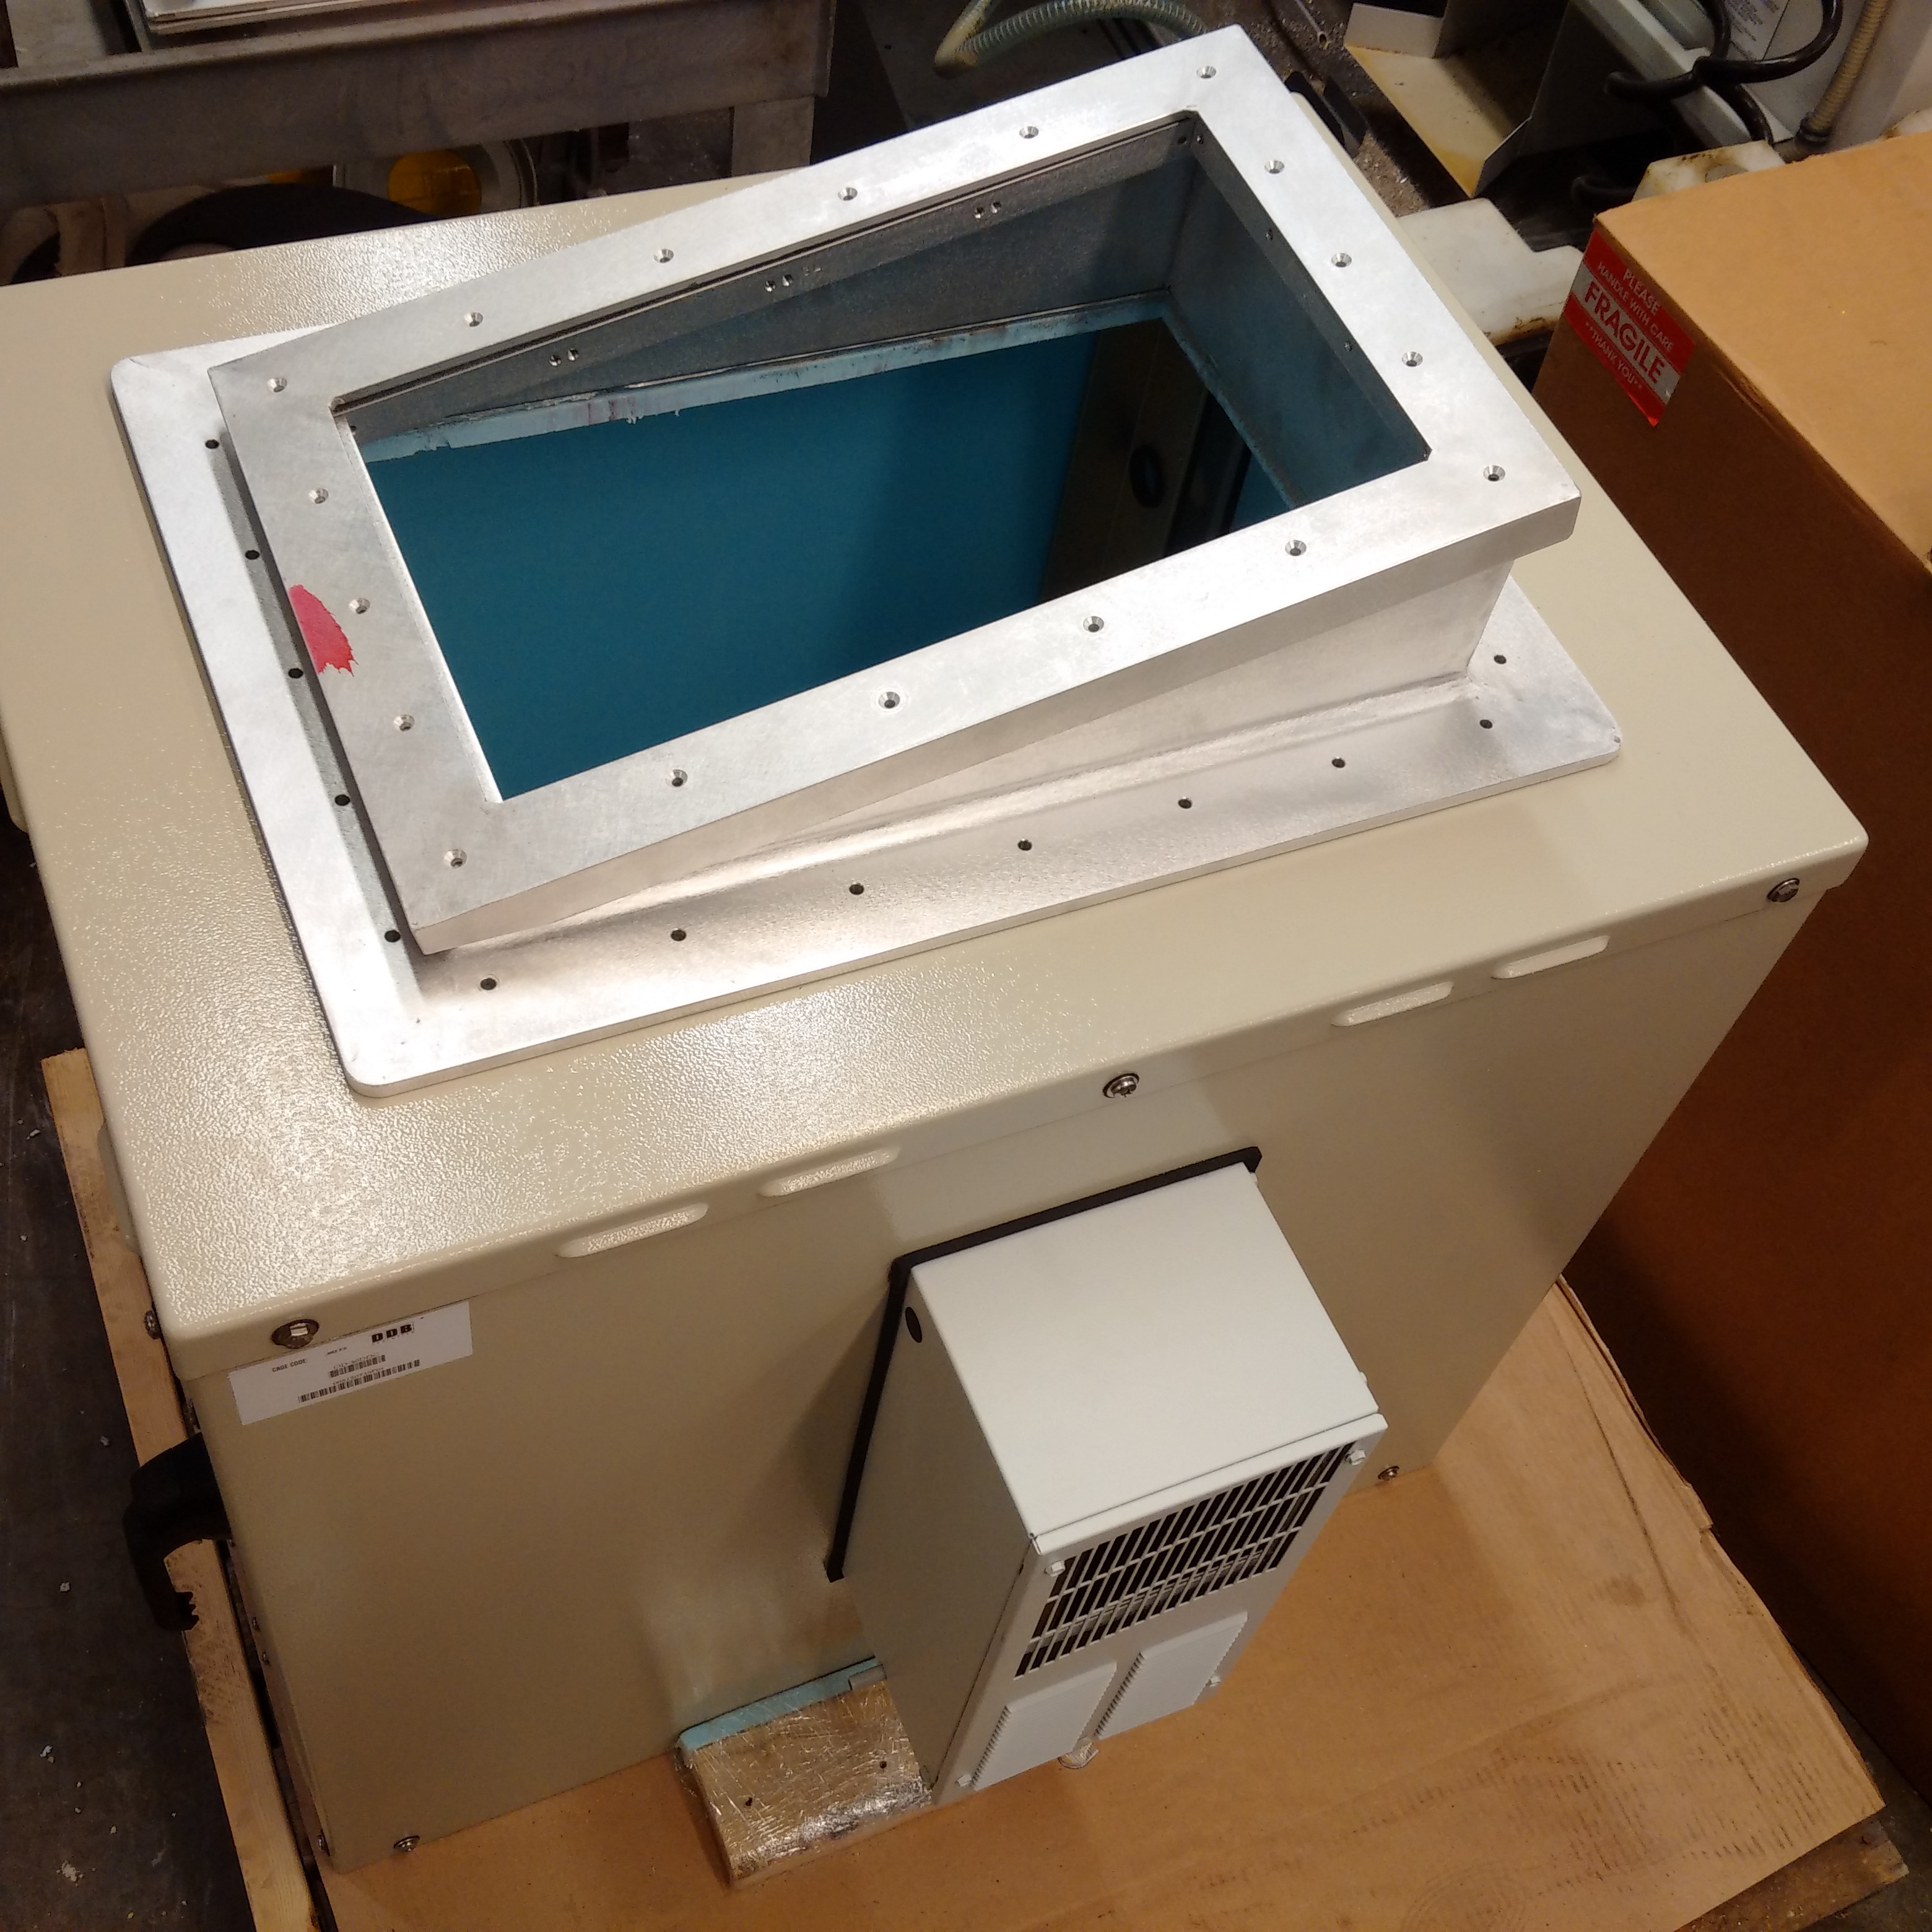
\includegraphics[width=\linewidth]{gfx/phase2cabinet}
	\caption{HiST Phase 2 cabinet with air conditioning as built in BU SIF.}
	\label{fig:hist2cab}
\end{figure}
This cabinet accommodates two cameras plus GPS and beacon receivers for enhanced data inversion via additional data inputs.
The next section describes the concerns involved with collecting and managing data from three to six cameras at remote unattended installations.

\FloatBarrier
\subsection{HiST Data}
A single camera in the HiST system collects over \unit[100]{GB} per hour, and given the remote unattended deployment of the cameras, substantial data reduction is necessary to avoid on-site human operation.
This reduction algorithm is described in detail in chapter~\ref{chapter:discrim}.
The data surviving this decision is further delineated by passing through the data inversion described in section~\ref{sec:inv}.

When using multiple instruments together to draw observational-based conclusions about the physics expressed by the phenomenon of interest, it is essential to know at least the relative timing error of each instrument. 
The HiST system employs GPSDOs at each camera site to yield timing accuracy $\ll \unit[1]{ms}$. 
Since this is a custom timing system, it is possible that errors in system design or equipment malfunction could cause an unexpected timing error. 
A convenient high temporal resolution test source in the common optical view are low earth orbit (LEO) satellites. 
LEO satellites are also easily visible with ISR in most modes of operation as bright targets > 10 times background.
Thus a tractable time verification can be achieved via an independent source--a geoscience instance of ``trust but verify''.
In particular, the Iridium constellation is a convenient candidate for time synchronization verification due to the large optical cross section and low orbit yielding an optically bright, fast-moving target. 
We must consider errors in SGP4 position propagation and ECI to azimuth and elevation (az/el) coördinate conversion.

The HiST geoscience optical instrument uses cameras including the Andor iXon 897 and iXon 888, with notional parameters described in Table~\ref{tab:ixonrate}. 
\begin{table}\centering
    \caption{Typical dataflow rates for high-speed auroral cameras.}\label{tab:ixonrate}
    \begin{tabular}{lllll}
        \toprule
        Camera & Resolution [pixels] & Bit depth [bits] & frame rate [Hz] & MB/sec \\
        \midrule
        iXon 897 & 512 x 512 & 16 & 50 & 26.2 \\
        iXon 887 & 512 x 512 & 14 & 30 & 15.7 \\
        \bottomrule
    \end{tabular}
\end{table}
It is important for experiment designers to note that camera datasheet frame rates are specified using conditions that are often unrealistic for the extended (many hours) observations typical in auroral observatories. 
By experiments in our lab, a derating of 5\% to 10\% is common for the Andor sCMOS and EMCCD cameras tested, with example sCMOS results shown in Table~\ref{tab:neomax}.
Even at the reduced frame rates in Table~\ref{tab:ixonrate}, imperfections in camera operations (e.g. dropped frames) were commonly observed, as often as multiple times per night.


A hardware monitor of the camera frame acquisition output accounts for any firmware glitches with regard to timing.
The deterministic counter in HiST shown in Figure~\ref{fig:histtime} uses the National Instruments PCIe-6321 with eight timers on an Application Specific Integrated Circuit (ASIC).
\begin{sidewaysfigure}\centering
    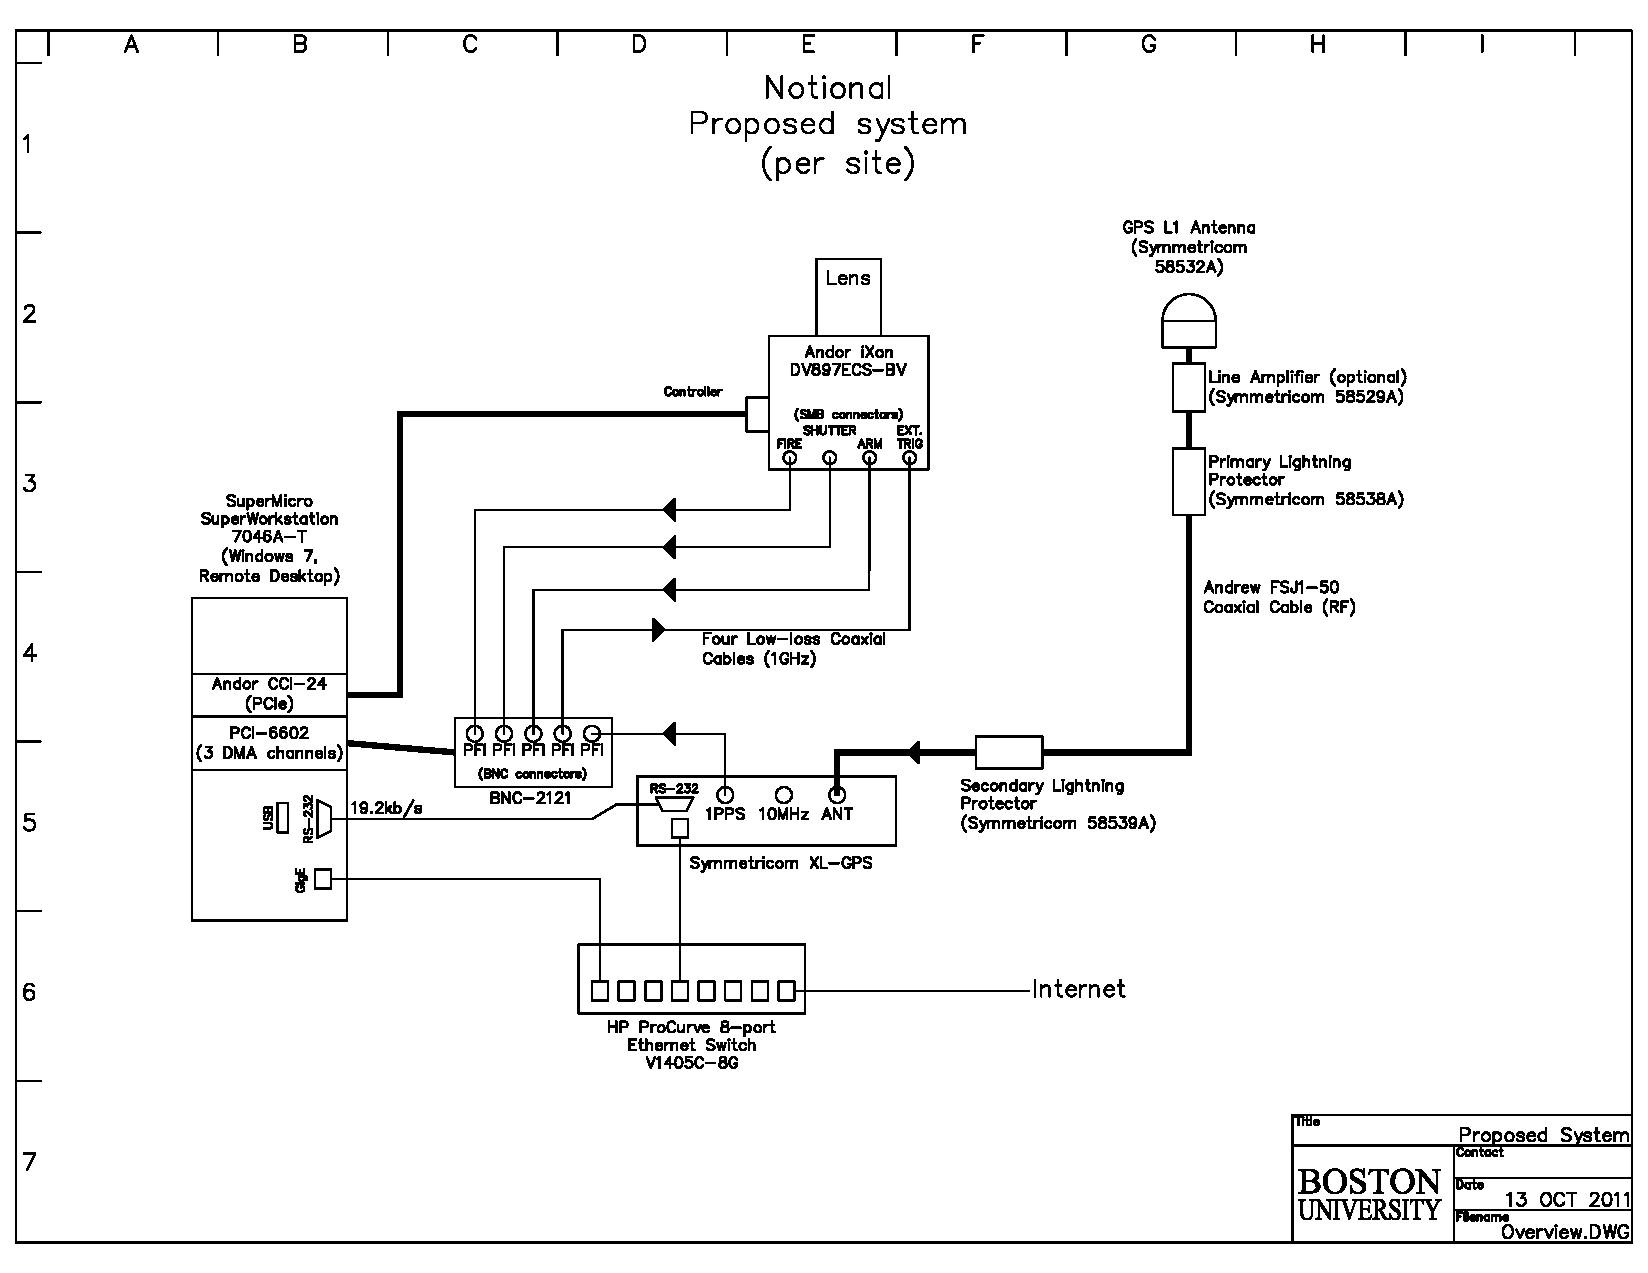
\includegraphics[page=1,width=0.95\linewidth]{gfx/ProposedTimingSystem}
    \caption{HiST timing system block diagram.}\label{fig:histtime}
\end{sidewaysfigure}
At the user's option, an additional deterministic timer per site is used to fire the cameras at precise intervals.
For simplicity and especially where the cameras are operated at distinct frame rates with a non-multiple relationship between the cameras, the cameras can be set to free run mode where the absolute time is recovered from the frame acquisition output.
In this manner, any camera with a frame acquisition binary output can be part of the HiST network.
Most scientific cameras with sufficient sensitivity have such an output.

The image collection software and hardware techniques developed in this dissertation are generalizable to any remote imaging system, and were used in developing the HiST Phase 2 instrument.
A map of candidate HiST Phase 2 sites (there will be three sites) is shown in Figure~\ref{fig:hist3}.
\begin{figure}
	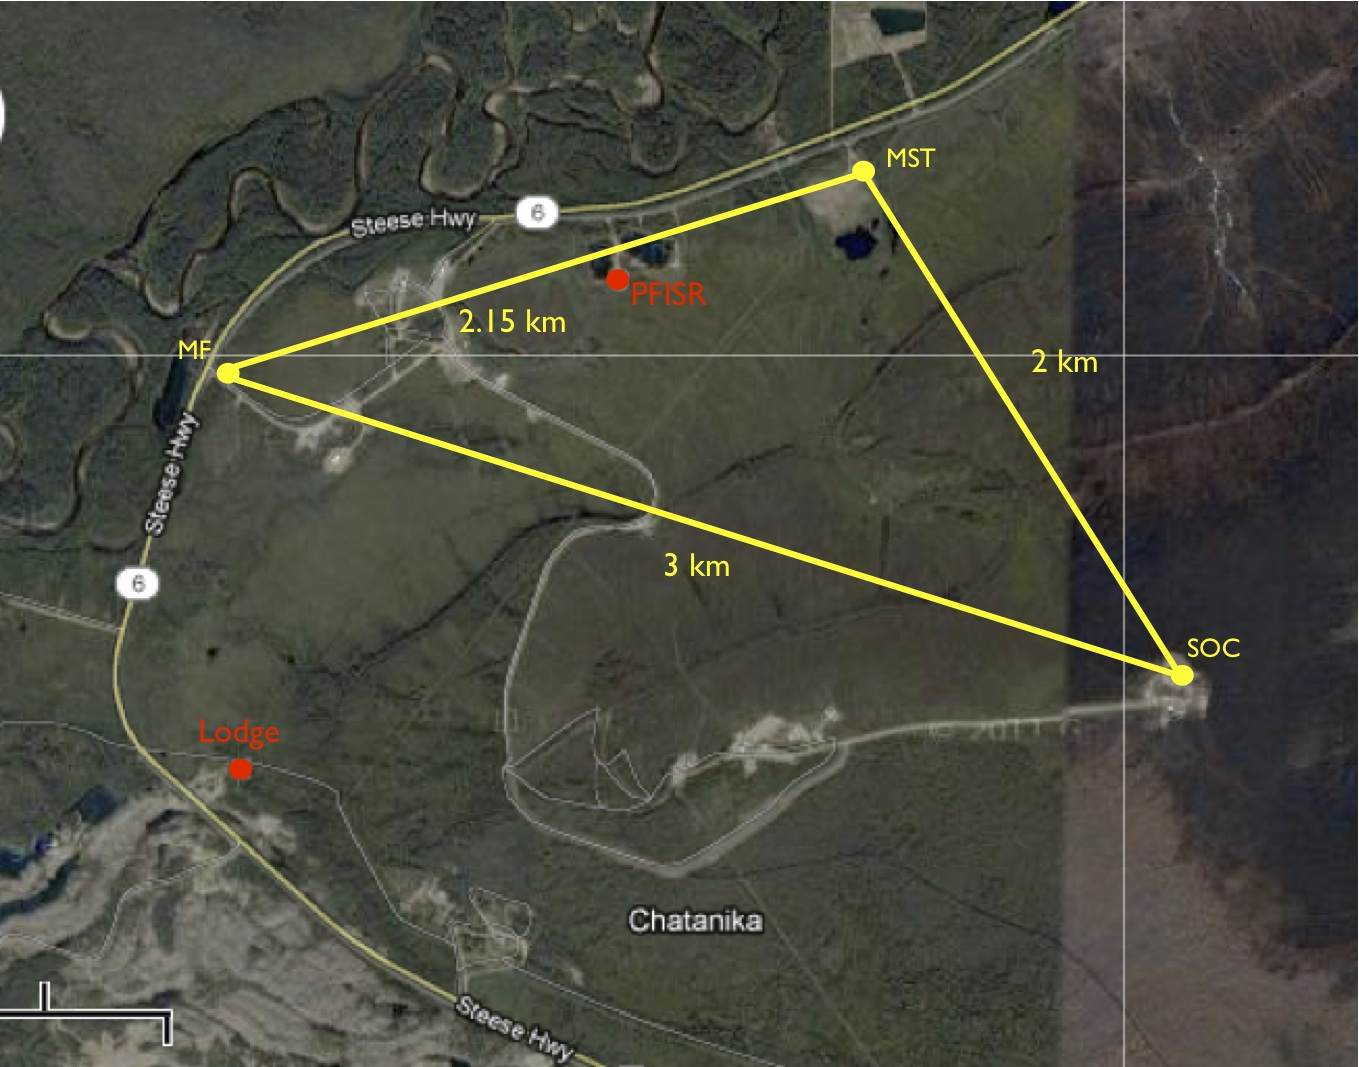
\includegraphics[width=\linewidth]{gfx/Optical_Sites3}
	\caption{Candidate sites for three site HiST Phase 2 deployment.}
	\label{fig:hist3}
\end{figure}
Initial processing will be with pairs of cameras, with the eventual goal of integrated three camera plus ISR data inversion.



%\FloatBarrier
\subsection{Poker Flat ISR (PFISR)}\label{sec:fuspfisr}
PFISR produces several low-level data products including the complex analog-to-digital converter voltage samples.
At the time, access to the large files containing low-level PFISR data is by request, with radar data accumulating at $\sim \unit[1.5]{MB/s}$ during a typical experiment.
% data: Apr 14 2013  (468530486 + 224263860 + 224263860 + 187839490) bytes / 729 seconds = 1.516 MByte/sec
Madrigal PFISR high-level data products have integration times $\sim \unit[2]{min}$ versus \unit[10..100]{ms} cadence of the low-level PFISR data.
Long integration time is necessary for plasma parameter estimation since incoherent returns from the ionospheric volume target provide return signals far too weak to characterize from a single pulse.
An autocorrelation function (ACF) is built up from the incoherent electron and ion scatterers over tens of seconds.
Taking the Fourier transform of the ACF the power spectral density (PSD) is obtained, with a notional PSD from a quiet ionosphere shown in Figure~\ref{fig:isrmorph}(a).
An ACF fitting algorithm provides estimates of electron number density, electron and ion temperature and ion velocity.

These plasma parameter estimates break down when turbulent plasma leads to a breakdown in the parameter fitter, which expects PSDs having morphology similar to Figure~\ref{fig:isrmorph}(a).
Strong Langmuir turbulence \citep{akbari2012} leads to ISR spectrum like that depicted in Figure~\ref{fig:isrmorph}(b).
\begin{figure}\centering
    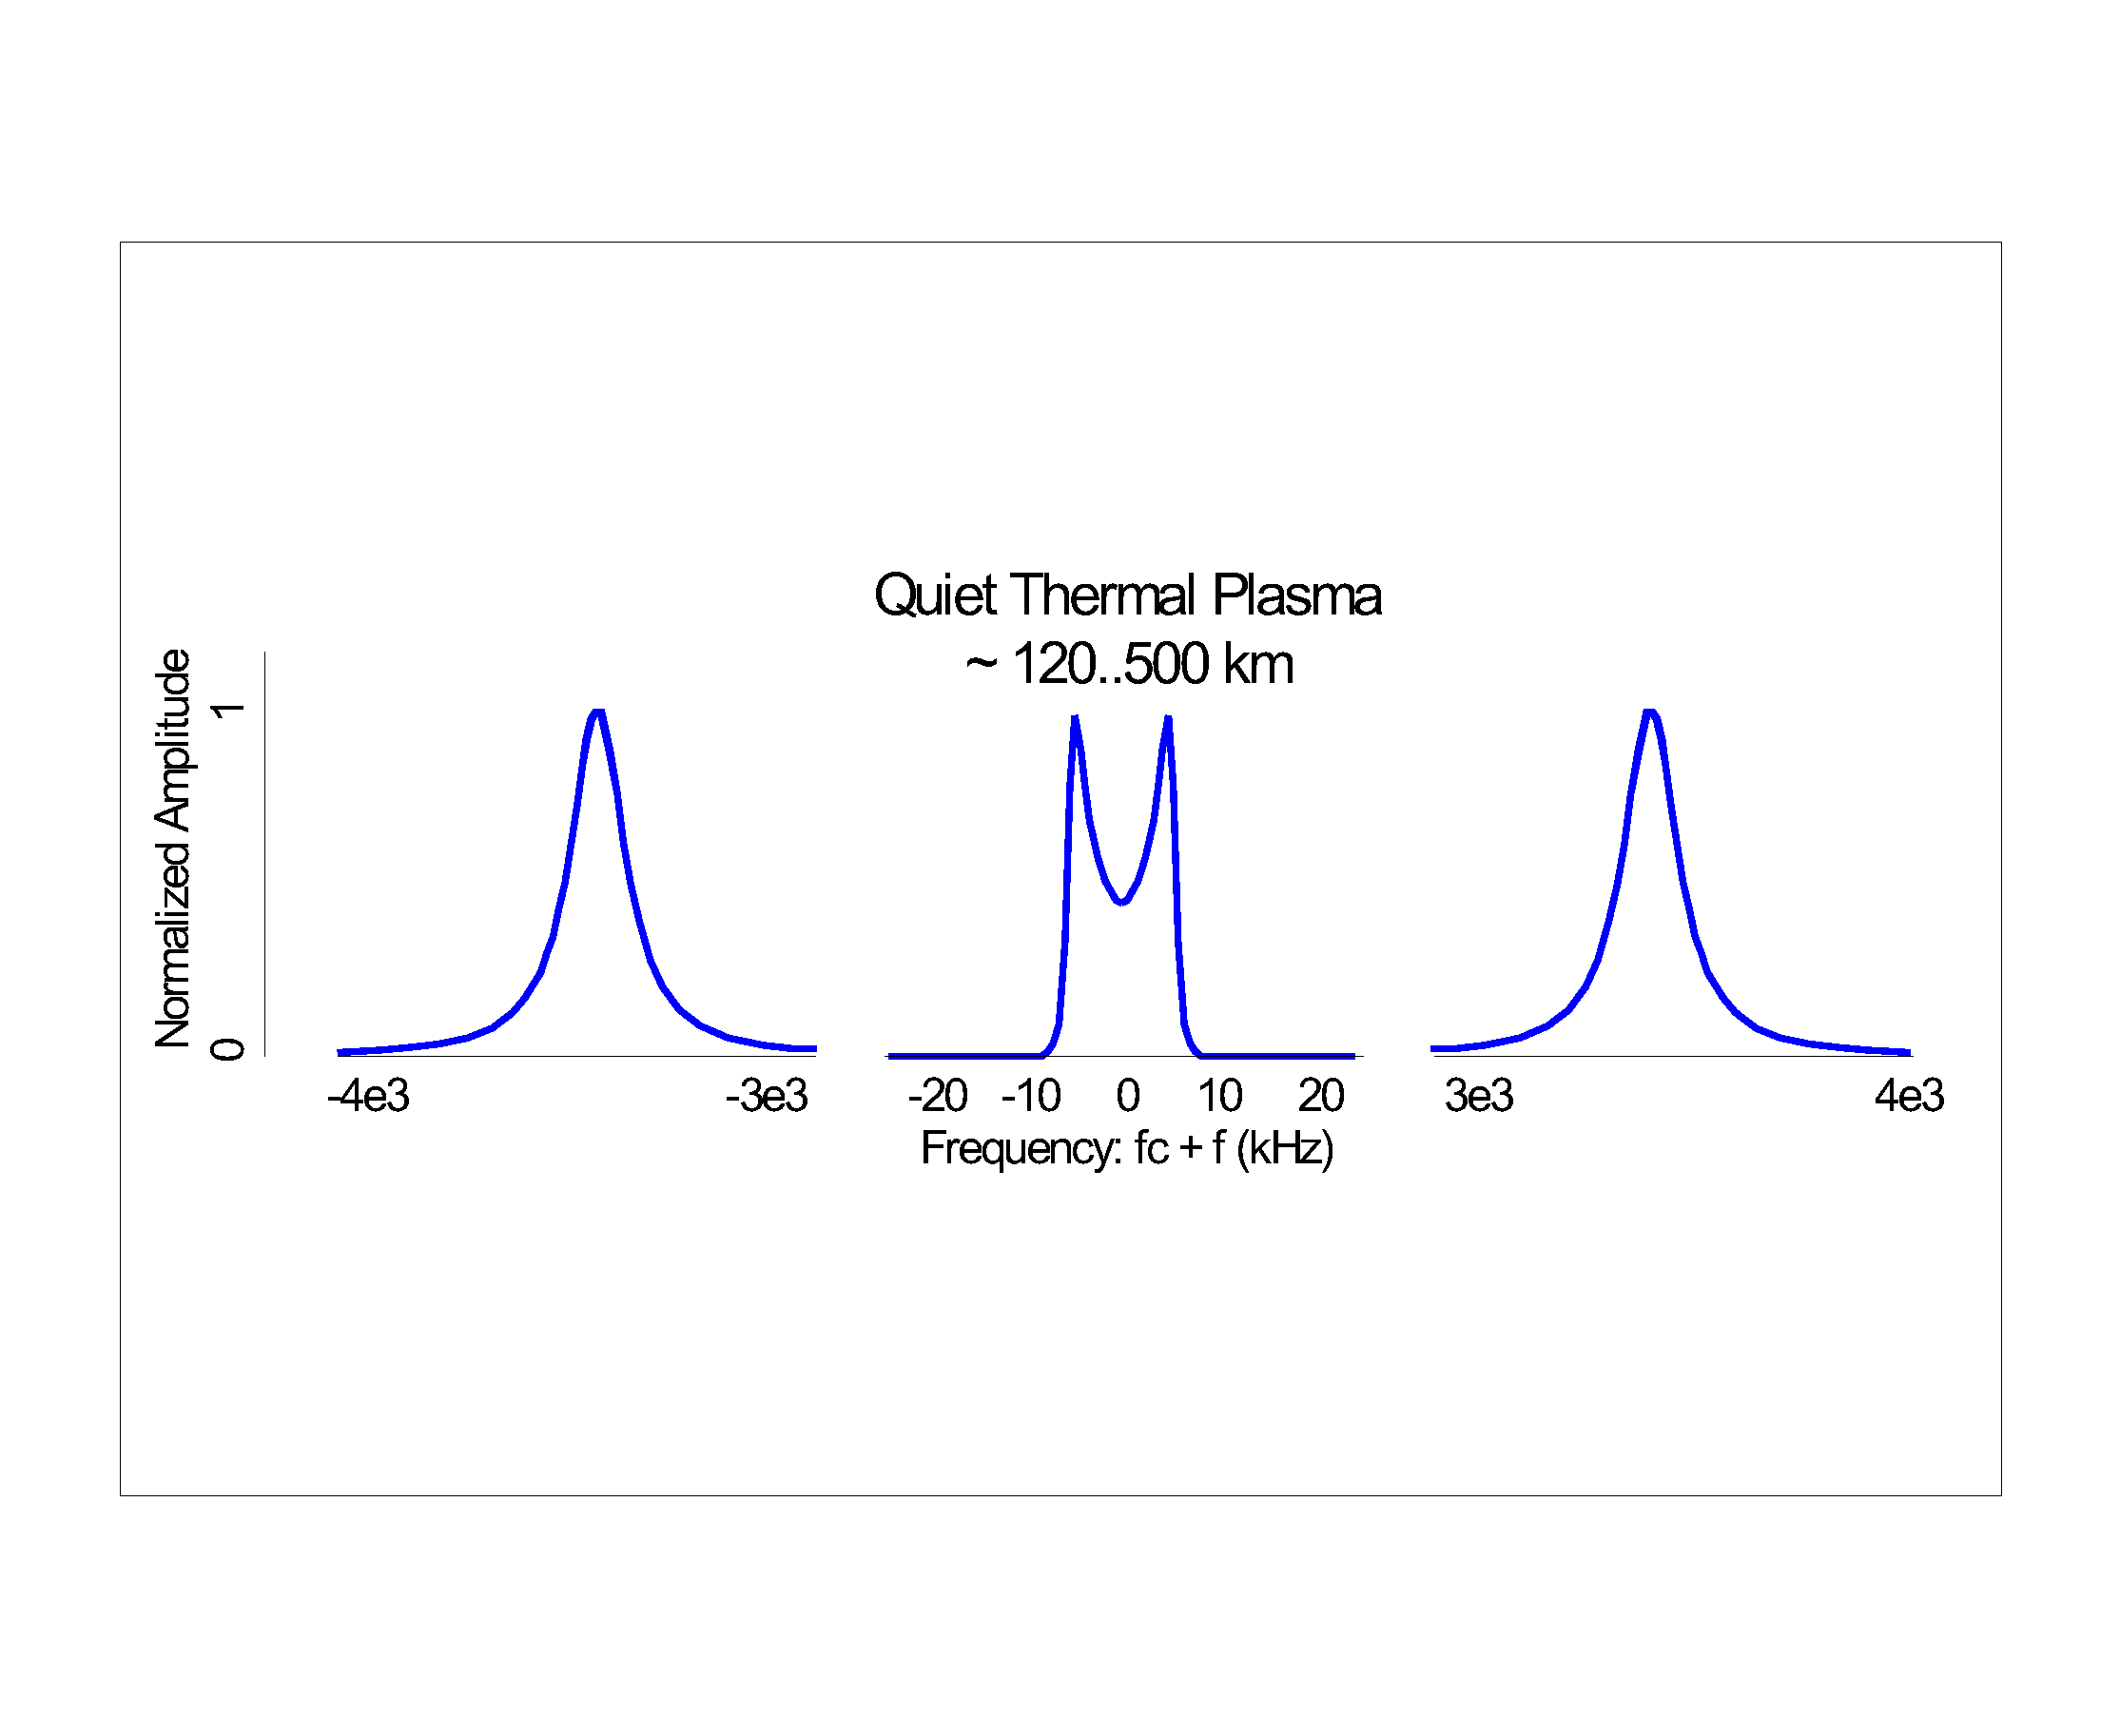
\includegraphics[width=0.8\columnwidth,trim=80 260 100 280,clip]{gfx/isr_thermal}

    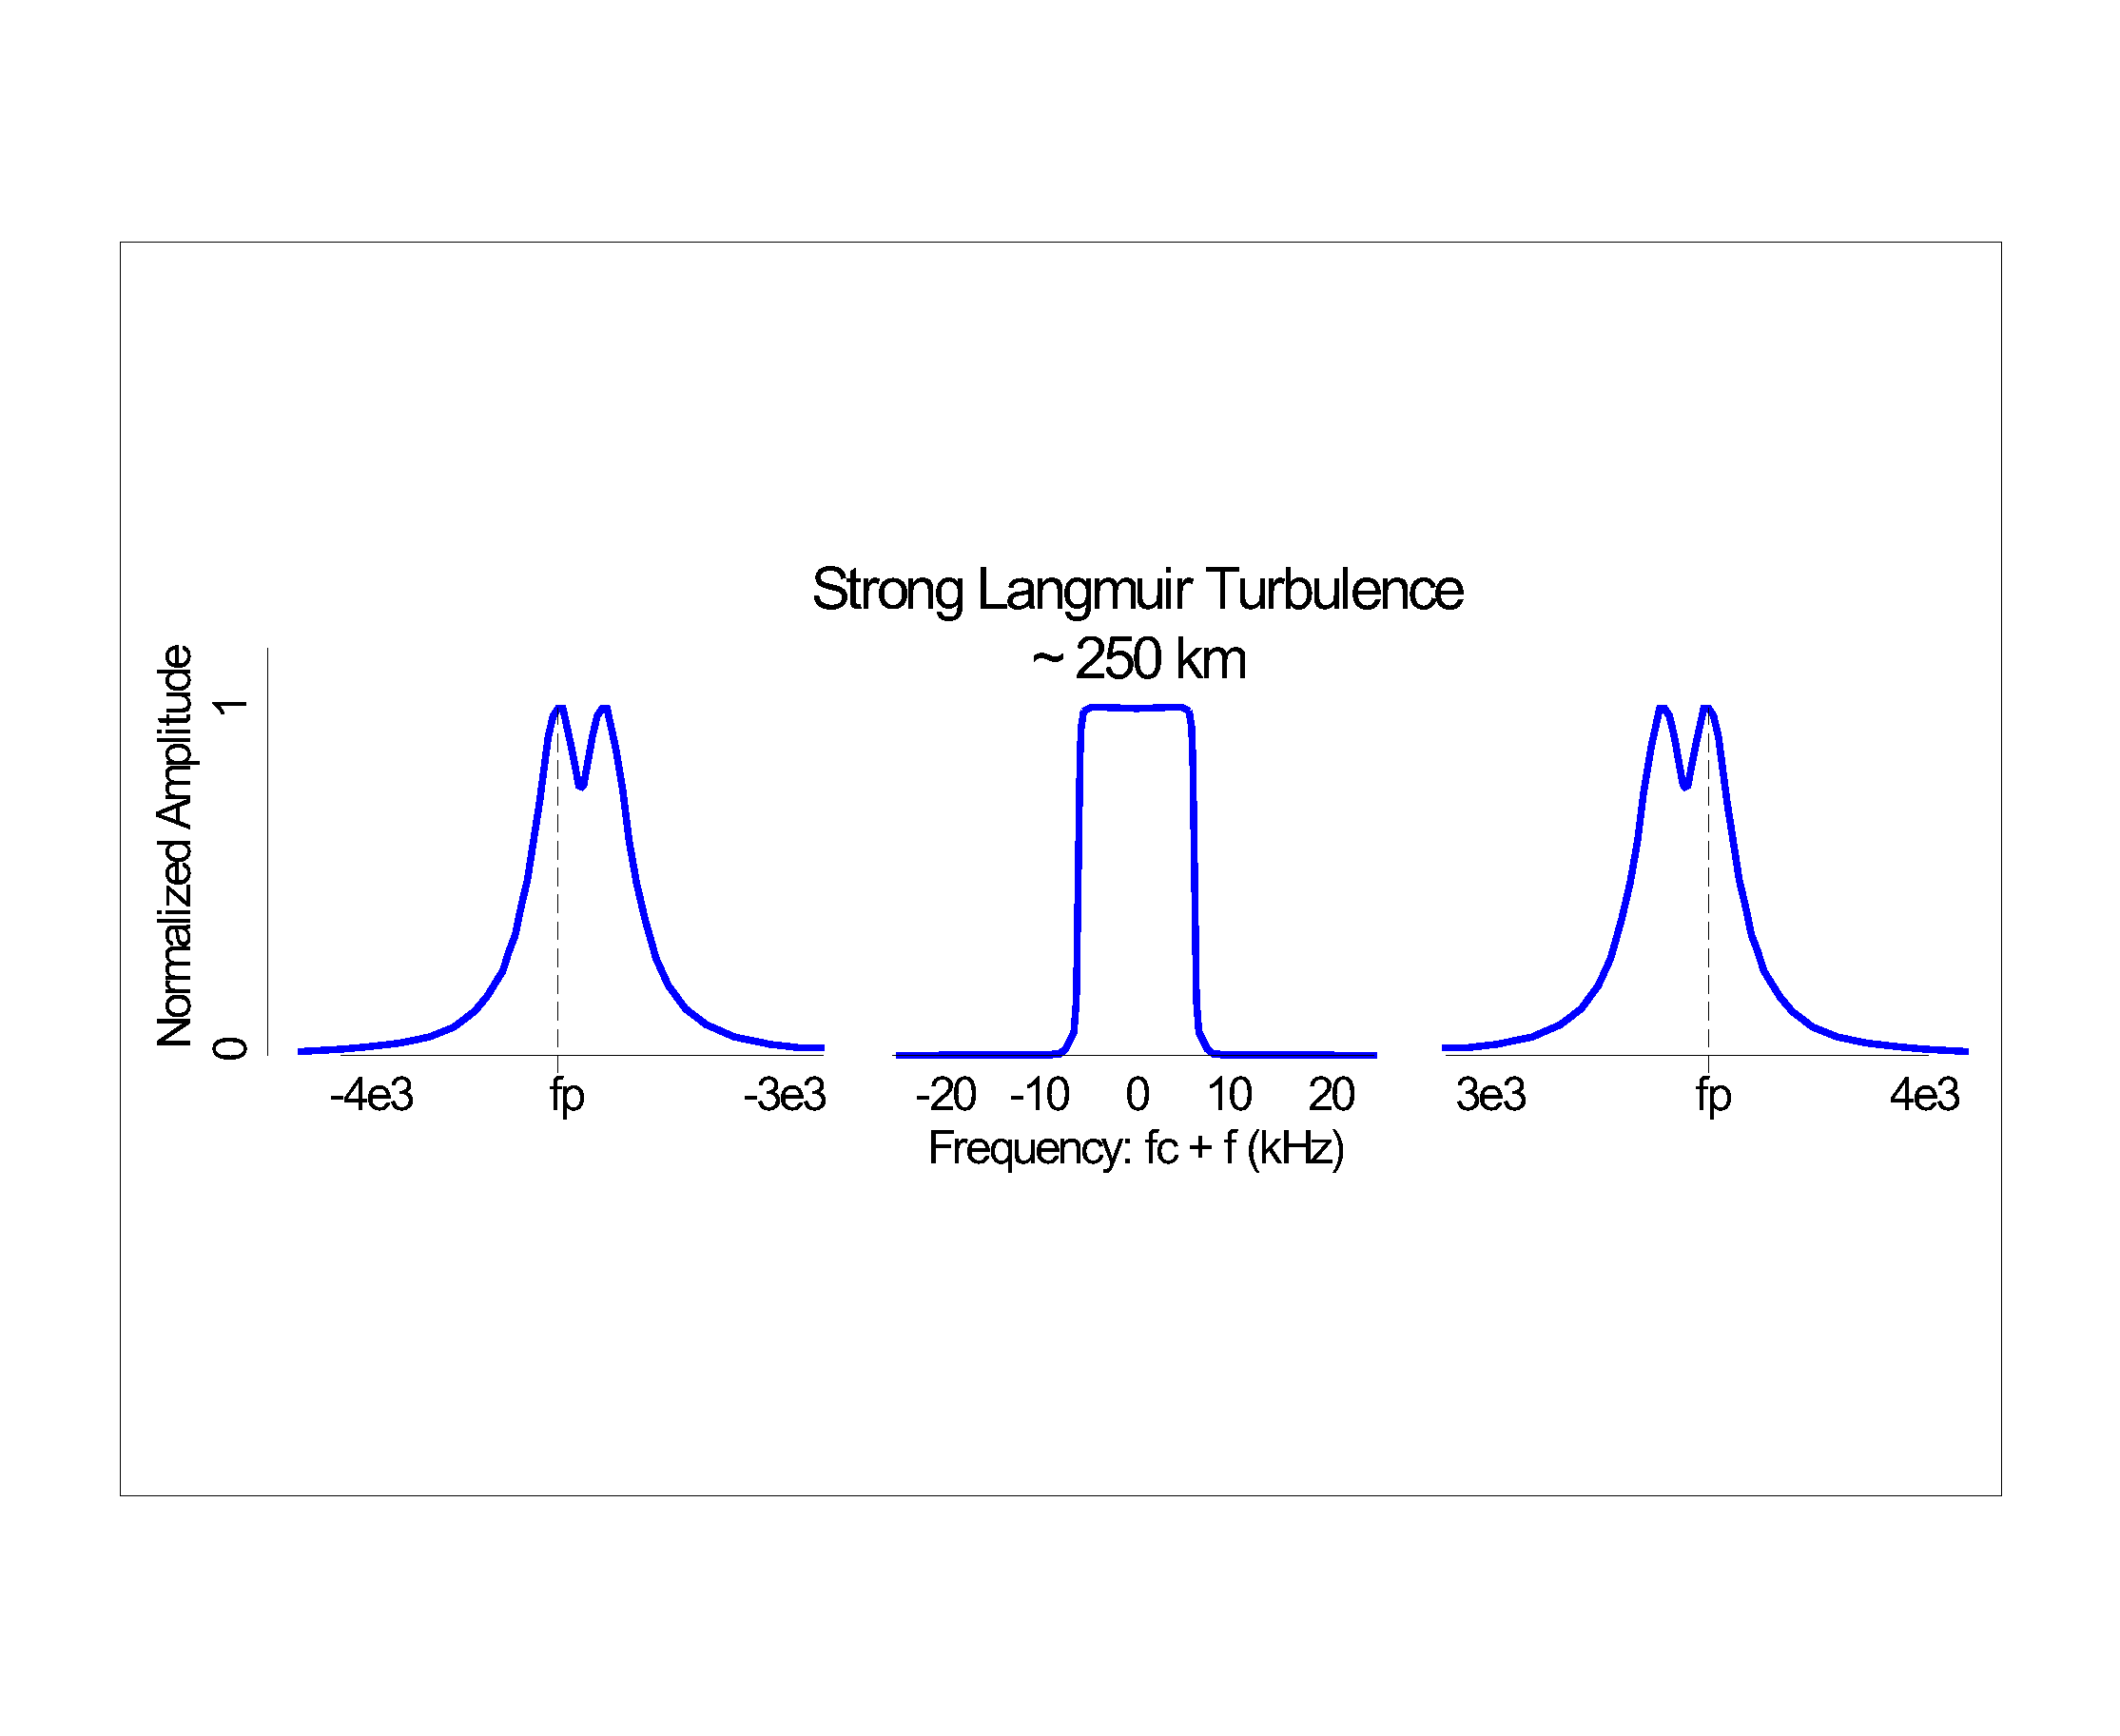
\includegraphics[width=0.8\columnwidth,trim=80 260 100 270,clip]{gfx/isr_slt}

    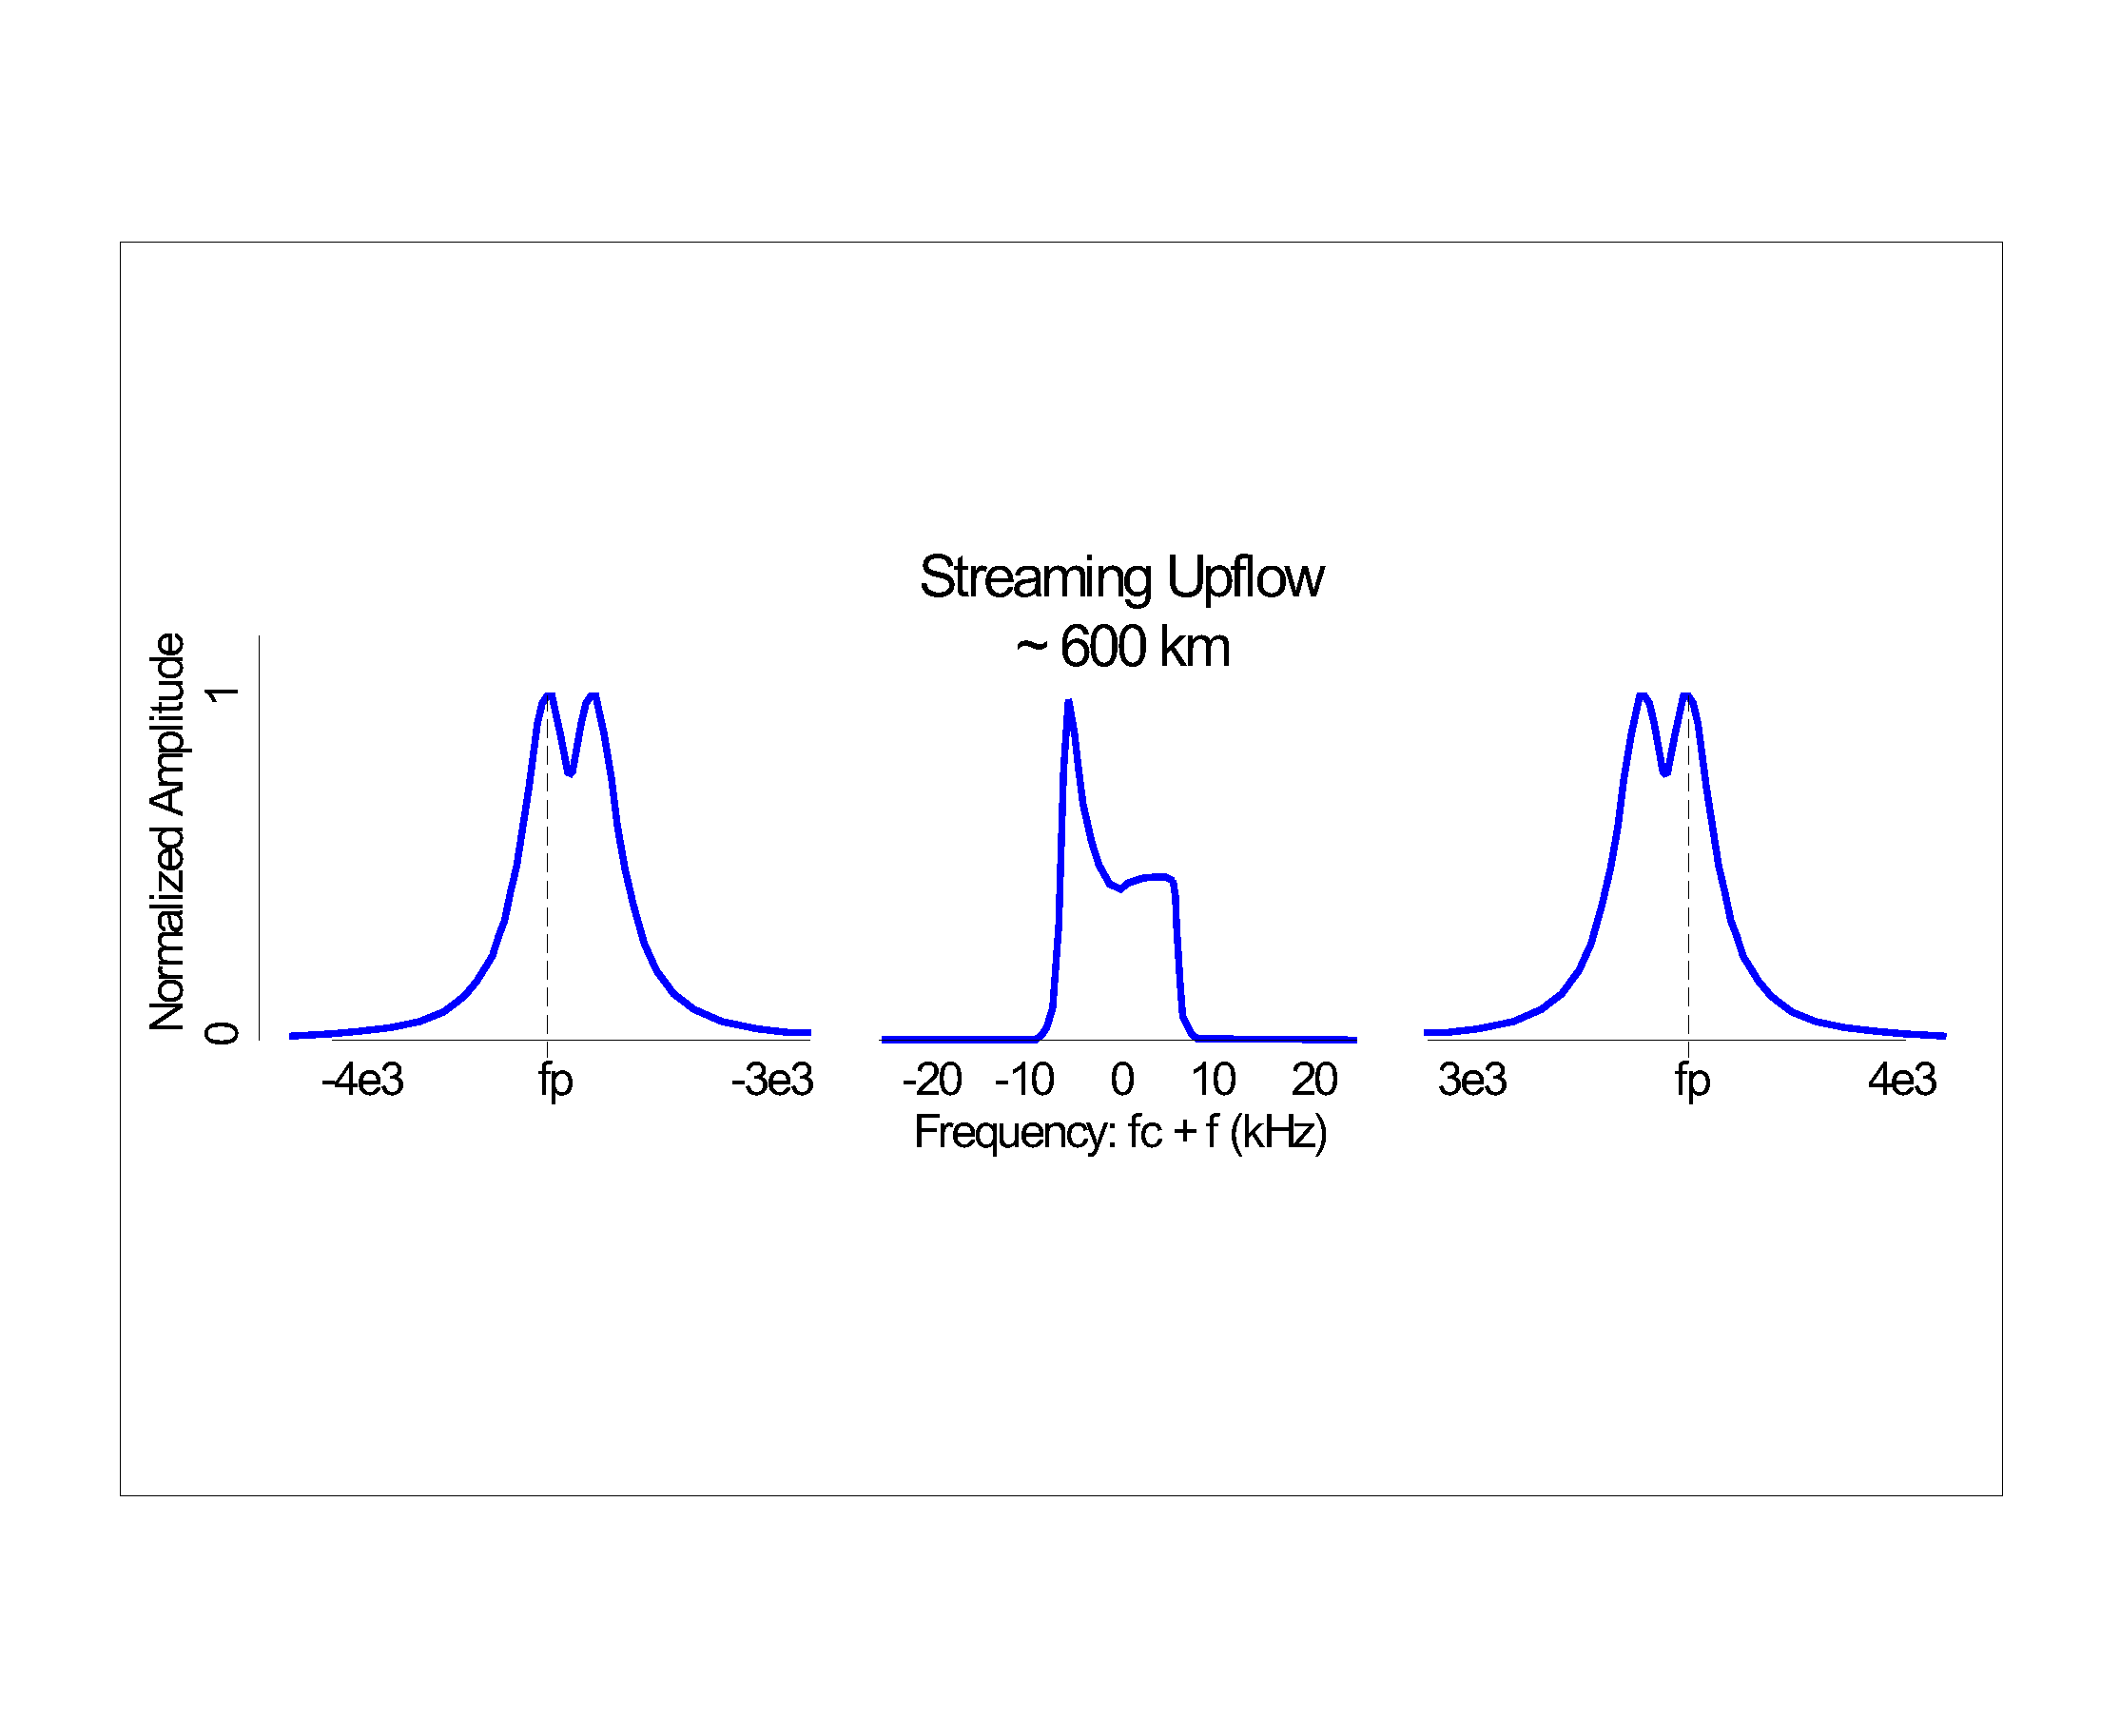
\includegraphics[width=0.8\columnwidth,trim=80 260 100 270,clip]{gfx/isr_streamupflow}
    \caption{(a) Notional PFISR spectrum for quiet ionospheric conditions. 
    	(b) Notional PFISR spectrum under strong Langmuir turbulence. 
    	(c) Notional PFISR spectrum with streaming upflowing plasma.}
    \label{fig:isrmorph}
\end{figure}
Streaming upflows lead to ISR spectrum similar to the depiction in Figure~\ref{fig:isrmorph}(c).
The ISR fitter algorithm used in plasma parameter estimation assumes a single-Maxwellian distribution, which breaks down under turbulent conditions, leading to non-physical plasma parameter estimates.
Alfvénic aurora associated with this Langmuir turbulence leaves fingerprints in the auroral morphology HiST was designed to observe.

The PFISR complex vector $\mathbf{I}+j\mathbf{Q}$ sampled time series is obtained with revisit time as fast as \unit[75]{ms} \citep{akbari2012} for five-beam pattern experiments and may be pushed at least to \unit[19]{ms} \citep{michell2009} for single-beam position experiments.
For future measurements, new ISR plasma line receiver techniques \citep{vierinen2016} reduce plasma line sampling cadence to about \unit[200]{ms}.
Table~\ref{tab:cadence} summarizes the time sampling capability of PFISR.
\begin{table}\centering
    \caption{Instrument sample rates vs. resolution used in experiments.}\label{tab:cadence}
    \begin{tabular}{llll}
        \toprule
        Instrument Measurement Mode & Resolution & Cadence [ms] & Date\\
        \midrule
        PFISR ion line long pulse & five beams    & 75   & 2011-03-01 \\
        PFISR plasma line long pulse & five beams & 6000 &  \\
        Andor Neo sCMOS camera & $1280 \times 1080$  & 20 &  \\
        \midrule
        PFISR ion line long pulse & 23 beams      & 234  & 2013-04-14 \\
        PFISR plasma line long pulse & 23 beams & 14000 &  \\
        Andor iXon EMCCD camera & $512 \times 512$ & 20 & \\
        \bottomrule
    \end{tabular}
\end{table}

Radar receive power for a beam-filling target may be described as
\begin{equation}
%P_r = K\frac{\tau_p P_t}{r^2}G_t G_r n_e \sigma
P_r = (F G_0) P_t L n_e \sigma c \tau \lambda^2 (64 \pi^2 r^2)^{-1} \textrm{[watts]}
\end{equation}
where $P_r$ is power received at the antenna terminals, $F$ is the antenna taper factor accounting for non-boxcar shape of beam, taken as 0.76 in \citet{evans1969}, $G_0$ is boresight antenna gain, $P_t$ is the power transmitted at the antenna terminals, $L$ is radar system losses, $\tau$ is the radar pulse length and $r$ is the one-way slant range to the measured range gate (alternatively called voxel or resolution cell).
The cross section of the beam-filling target is \citep{nicolls2015,evans1969}
\begin{equation}
\sigma = \frac{\sigma_e}{(1+\alpha^2)(1+\frac{T_e}{T_i} + \alpha^2)}
\end{equation}
where $\alpha = 4\pi \lambda_D / \lambda$, the radar cross section of an electron is 
\begin{equation}
\sigma_e = 4 \pi(r_e \sin \psi)^2
\end{equation}
the electron radius is
\begin{equation}
r_e = \frac{e^2}{\varepsilon_0 m_e c^2}
\end{equation}
and $\psi=\pi/2$ for a backscattered electron \citep{evans1969}.
For computing SNR, the noise power is
\begin{equation}
P_n = k_B T_s B
\end{equation}
where $T_s$ is system temperature.
The ISR PSD shape is a function involving many terms, and the reader is referred to \citet{evans1969} equations (18-21) for the specifics.


PFISR ion-line PSD is obtained by taking the Fourier transform of the autocorrelation function.
The ion line spectra are typically observed as two equal-amplitude frequency-smeared impulses symmetric about the radar center frequency.
Typical Doppler bandwidth is less than \unit[25]{kHz} for the \unit[450]{MHz} AMISR.
PFISR plasma-line spectra are shifted several MHz up and down from the radar center frequency, so a slice of the receiver spectrum is extracted where the plasma lines are expected to occur to conserve data and storage resources.
Under quiet and inverted-V auroral conditions, the ISR ion-line spectrum assumptions made by the fitter are fulfilled.
Using assumptions on atmospheric composition (species and density) vs. altitude, an least squares fit of the ion-line PSD is made to estimate the plasma parameters $N_e, T_e, T_i, V_i$.
Further consideration of the fitting of plasma parameters to the ion-line spectrum is given in \citet{swobodathesis}.


A summing-over-altitude technique is useful in both the ion line and plasma line data as a method to draw out weaker coherent returns not otherwise visible.
We integrate $P_r$ in the NEIAL altitude range of roughly \unit[200..400]{km} and plot this integrated measurement as a time series with a representative NEIAL event in Figure~\ref{fig:shedintion}.
\begin{figure}
    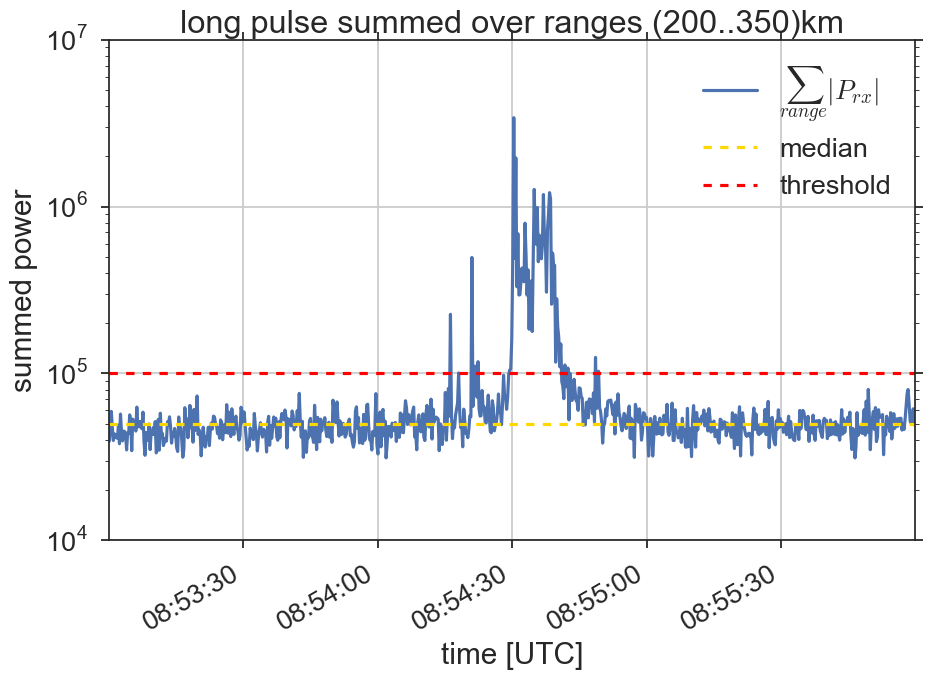
\includegraphics[width=0.9\columnwidth]{gfx/2013-04-14T0854/summedAlt2013-04-14T08-54}
    \caption{Receive power of Figure~\ref{fig:20130414T0854a}(e) integrated over \unit[200..350]{km}. 
        Observe turbulence perturbation from approximately 8:54-8:55~UT.}
    \label{fig:shedintion}
\end{figure}
Considering the large amount of raw data collected each day, a method of automated turbulence detection is quite useful, particularly during daylight hours when auroral video is not available.
Cell-median CFAR is the method used in this work.
\citet{schlatter2014} used image processing techniques to further restrict ``matching'' events. 
In contrast, the goal in this work was to achieve high sensitivity and manually filter out spurious events such as satellites.
Most of the time turbulence does not occur, so we can use the median of the last $N$ measurements and set a threshold based on a constant $K$ factor above this rolling median $\widetilde{M}$.
Using Figure~\ref{fig:shedintion} as an example, suppose the rolling median is 50,000.
We can decide detection by
\begin{equation}\label{eq:cfarsum}
S \gtrless K\cdot\widetilde{M}
\end{equation}
based on summed power $S$ vs $K=2.0$ as the threshold factor in this example.


%\section{Digital All-Sky Camera (DASC)}
The DASC instrument has a $360^\circ$ azimuthal view at elevations from horizon to local geographic zenith at $512 \times 512$ pixel resolution. 
When interpreting DASC images, unwarping using \citet{geodata} shows video on the computer screen as it would appear to a human observer looking at the sky, helping eliminate the massive barrel distortion inherent to all-sky images.
On 14 APR 2013, DASC took an image at each of $\lambda \in \lbrace 427.8, 557.5, 630.0 \rbrace$~nm approximately every \unit[13]{s}.
Previous work has combined the three image channels into a pseudo-RGB image, but the issue of temporal aliasing is noted for dispersive auroral events, since each color channel is obtained with about \unit[4]{s} spacing.
%We present the DASC images in three columns by wavelength.
Note that the HiST instrument by design highly attenuates \unit[557.7]{nm} and \unit[630.0]{nm} emissions, while the prompt \unit[427.8]{nm} emission is one of the primary emissions observed by HiST.



